%
% note line 490, 603, 388, 409
%
\chapter{Homoclinic Bifurcation of a Rod in a Magnetic Field} \label{chap:bifurcation}
%
\par % Intro
Having derived homoclinics in the unperturbed integrable case and proved the existence of multimodal homoclinics in perturbed nonintegrable cases, in this chapter homoclinic solutions shall be constructed and their bifurcation structure investigated for both primary and multimodal configurations.
% 
\par % overview of technical detail
The computation of homoclinic solutions requires that the arclength be truncated from the infinite domain $s \in \left(-\infty,+\infty\right)$ to the interval $s \in \left[0,\mathcal{T}\right]$. The computation of homoclinics then becomes a boundary value problem where the left-hand side conditions are placed in the unstable mainfold of the trivial equilibrium and the right-hand side conditions satisfy a reversibility. By using the Newton-Raphson method to solve a variational equation with respect to a set of shooting parameters at each iteration, the boundary value problem is then solved using a shooting method. Due to the magnetic effects the system investigated in this chapter is nongeneric as the trivial solution is a periodic orbit, so specific details of the computation and continuation of homoclinic particular to this system are explained. For further details on the computation and continuation of homoclinic solutions in a more general case see appendix~\S\ref{chap:numerics}. 
%
\par % Introduce Euler parameters
In order to increase the computational efficiency the four Euler parameters $q~=~\left(q_{1},q_{2},q_{3},q_{4}\right)$ are used to reduce the dimension of the system. The rotation matrix~\eqref{eq:frame} is then given by
%
\begin{align}
R & = 
\left(
\begin{array}{ccc}
q_{1}^{2} - q_{2}^{2} - q_{3}^{2} + q_{4}^{2} & 2\left(q_{1}^{}q_{2}^{} - q_{3}^{}q_{4}^{}\right) & 2\left( q_{1}^{}q_{3}^{} + q_{2}^{}q_{4}^{} \right) \\
2\left(q_{1}^{}q_{2}^{} + q_{3}^{}q_{4}^{} \right) & q_{2}^{2} + q_{4}^{2} - q_{1}^{2} - q_{3}^{2} & 2\left(q_{2}^{}q_{3}^{} - q_{1}^{}q_{4}^{} \right) \\
2\left(q_{1}^{}q_{3}^{} - q_{2}^{}q_{4}^{} \right) & 2\left(q_{1}^{}q_{4}^{} - q_{2}^{}q_{3}^{} \right) & q_{3}^{2} + q_{4}^{2} - q_{1}^{2} - q_{2}^{2}
\end{array}
\right). \label{eq:ep}
\end{align}
%
The four Euler parameters give a double covering of the set of rotations subject to the constraint 
%
\begin{align}
{q}\cdot{q} = q_{1}^{2} + q_{2}^{2} + q_{3}^{4} + q_{4}^{2} & = 1. \label{eq:ep_Casimir}
\end{align}
%
The Euler parameters are robust in that unlike the Euler angles there is no polar singularity. They are a projection of the phase space onto the surface of a four-dimensional unit sphere. For more details on the Euler parameters and their relation to the Euler angles see appendix~\S\ref{chap:parameterisation}.
% 
\par % e_{3}
From~\eqref{eq:ep} the triple $\mathsf{e}_{1}$ becomes a function of the Euler parameters. 
%
\begin{align}
\mathsf{e}_{3}\left(q\right) & = \left( \begin{array}{c}
2 \left( q_{1}^{}q_{3}^{} + q_{2}^{}q_{4}^{} \right) \\
2 \left( q_{2}^{}q_{3}^{} - q_{1}^{}q_{4}^{} \right) \\
q_{3}^{2} + q_{4}^{2} - q_{1}^{2} - q_{2}^{2}
\end{array}\right).
\label{eq:e3_ep}
\end{align}
% 
\par % Strains
From~\eqref{eq:curvatures} the strains can be written as
%
\begin{align}
u_{i} & = \frac{ 2 \, B_{i} \, q \cdot q^{\prime}}{ q \cdot q } \quad \mbox{for} \quad i=1,2,3 \label{eq:euler_strains}
\end{align}
%
where the ${B}_{i}$ are four-by-four skew-symmetric matrices satisfying the relationships
%
\begin{align}
B_{1}q & = \left( q_{4}, q_{3}, -q_{2}, -q_{1} \right), \nonumber \\
B_{2}q & = \left( -q_{3}, q_{4}, q_{1}, -q_{2} \right), \nonumber \\
B_{3}q & = \left( q_{2}, -q_{1}, q_{4}, -q_{3} \right). \nonumber
\end{align}
%
The four vectors $\left\{ q, B_{1}q, B_{2}q, B_{3}q \right\}$ form an orthonormal basis in $\mathbb{R}^{4}$. Thus~\eqref{eq:euler_strains} subject to~\eqref{eq:ep_Casimir} can be inverted and solved for the derivatives of the Euler parameters as
%
\begin{subequations}
\label{eq:ep_evolution}
\begin{align}
q_{1}^{\prime} & = \left( u_{1}q_{4} - u_{2}q_{3} + u_{3}q_{2} \right)\slash{2},\\
q_{2}^{\prime} & = \left( u_{1}q_{3} + u_{2}q_{4} - u_{3}q_{1} \right)\slash{2},\\
q_{3}^{\prime} & = \left(-u_{1}q_{2} + u_{2}q_{1} + u_{3}q_{4} \right)\slash{2},\\
q_{4}^{\prime} & = \left(-u_{1}q_{1} - u_{2}q_{2} - u_{3}q_{3} \right)\slash{2}.
\end{align}
\end{subequations}
% 
Thus, the formulation of the governing equations based on the force and moment balance equations~\eqref{eq:magnetic_moment},~\eqref{eq:magnetic_force} with the constraint~\eqref{eq:ep_evolution} and body force~\eqref{eq:e3_ep} is a dynamical system of the form
%
\begin{align}
\boldsymbol{x}^{\prime} & = f \left(\boldsymbol{x}, \mu \right), \quad \boldsymbol{x} \in \mathbb{R}^{10} \quad \mbox{and} \quad \mu \in \mathbb{R}^{p}, \label{eq:equation}
\end{align}
%
where $p$ is the number of independent nondimensional parameters under consideration. 
%
\par % Boundary Conditions and nondimensionisation
It is assumed that a moment, $M$, and tension, $T$, are applied axially at $s=\pm\infty$. For simplicity let the constitutive relations take the form
%
\begin{equation}
u_{1} = m_{1}\slash B, \quad u_{2} = m_{2} \slash B, \quad u_{3} = m_{3}\slash C \quad \mbox{and} \quad v_{3} = 1 + n_{3}\slash J.
\end{equation}
% 
The system is then nondimensionalised by
%
\begin{equation}
\begin{array}{c}
t = \left(M\slash B\right) s, \quad x_{1} = n_{1}\slash{T},\quad x_{2} = n_{2}\slash{T},\quad x_{3} = \left(n_{3}-T\right)\slash{T},\\
x_{4} = m_{1}\slash{M},\quad x_{5} = m_{2}\slash{M},\quad x_{6} = \left(m_{3}-M\right)\slash{M},\\
x_{7}=q_{1}, \quad x_{8}=q_{2}, \quad x_{9}=q_{3}, \quad x_{10}=q_{4}. \\
\end{array}
\end{equation}
%
The nondimensional parameters for an extensible rod are then given by
%
\begin{equation}
m = \frac{M}{\sqrt{BT}}, \quad \bar\lambda = \frac{\lambda B}{M}, \quad \nu = \frac{B}{C}-1 \quad \mbox{and} \quad \epsilon = \frac{T}{J}.
\end{equation}
%
The nondimensional parameters are the same as those in~\eqref{eq:nondim} with the additional parameter $\bar\lambda$ as the unified magnetic body force parameter. The bar notation is suppressed from this point onwards. Thus, explicitly the governing equations are
%
\begin{subequations}
\label{eq:ge_full}
\begin{align}
x_{1}^{\prime}  & = \left( 1 + \nu \right)x_{2}x_{6} - x_{3}x_{5} + 2 \lambda\left(1+\epsilon x_{3}\right)\left( x_{7}x_{10} + x_{8}x_{9}\right), \\
x_{2}^{\prime}  & = x_{3}x_{4} - \left(1+\nu\right)x_{1}x_{6} - 2\lambda\left(1+\epsilon x_{3}\right)\left(x_{7}x_{9}-x_{8}x_{10}\right), \\
x_{3}^{\prime}  & = x_{1}x_{5} - x_{2}x_{4}, \\
x_{4}^{\prime}  & = \nu x_{5}x_{6} + x_{2}\left( 1 + \epsilon x_{3} \right) \slash m^{2}, \\
x_{5}^{\prime}  & =-\nu x_{4}x_{6} - x_{1}\left( 1 + \epsilon x_{3} \right) \slash m^{2}, \\
x_{6}^{\prime}  & = 0, \\
x_{7}^{\prime}  & = \left( x_{4}x_{10} - x_{5}x_{9} + \left(1+\nu\right)x_{6}x_{8} \right)\slash{2}, \\
x_{8}^{\prime}  & = \left( x_{4}x_{9} + x_{5}x_{10} - \left(1+\nu\right)x_{6}x_{7} \right)\slash{2},\\
x_{9}^{\prime}  & = \left(-x_{4}x_{8} + x_{5}x_{7} + \left(1+\nu\right)x_{6}x_{10} \right)\slash{2},\\
x_{10}^{\prime} & = \left(-x_{4}x_{7} - x_{5}x_{8} - \left(1+\nu\right)x_{6}x_{9} \right)\slash{2}.
\end{align}
\end{subequations}
%
It is a straight-forward exercise to check that the Casimirs~\eqref{eq:magnetic_casimirs}, 
%
\begin{subequations}
\label{eq:nondim_casimirs}
\begin{align}
\dfrac{1}{2} x_{1}^{2} + \dfrac{1}{2} x_{2}^{2} + \dfrac{1}{2} x_{3}^{2} +  2 \lambda x_{4} \left( x_{7}x_{9} + x_{8}x_{10} \right) + 2 \lambda x_{5} \left( x_{8}x_{9} - x_{7}x_{10} \right) \nonumber \\
\hspace{1.0cm} + \lambda x_{6} \left( x_{10}^{2}+x_{9}^{2}-x_{8}^{2}-x_{7}^{2} \right) & = \dfrac{1}{2} + \lambda, \label{eq:nondim_casimir_1} \\
x_{1} \left(  x_{7}x_{9} + x_{8}x_{10} \right) + x_{2} \left( x_{8}x_{9} - x_{7}x_{10} \right) + x_{3} \left( x_{10}^{2}+x_{9}^{2}-x_{8}^{2}-x_{7}^{2} \right) & =1, \label{eq:nondim_casimir_2} \\
\left( x_{7}x_{9} + x_{8}x_{10}\right)^{2} + \left( x_{8}x_{9} - x_{7}x_{10}\right)^{2} + \left( x_{10}^{2}+x_{9}^{2}-x_{8}^{2}-x_{7}^{2}\right)^{2} & = 1, \label{eq:nondim_casimir_3}
\end{align}
\end{subequations}
%
first integrals~\eqref{eq:magnetic_integrals} 
%
\begin{subequations}
\label{eq:nondim_integrals}
\begin{align}
x_{6} & = 1, \label{eq:nondim_integral_1} \\
x_{1} x_{4} + x_{2} x_{5} + x_{3} x_{6} +  \lambda \left( x_{10}^{2}+x_{9}^{2}-x_{8}^{2}-x_{7}^{2} \right) & = 1 + \lambda \label{eq:nondim_integral_2}
\end{align}
\end{subequations}
%
and constraint~\eqref{eq:ep_Casimir} 
%
\begin{align}
 x_{7}^{2} + x_{8}^{2} + x_{9}^{2} + x_{10}^{2} & = 1 \label{eq:nondim_constraint}
\end{align}
%
are all conserved quantities.
%
\par % Periodicity
The periodic orbit, with period given by $\tau = 2\pi\slash\left(1+\nu\right)$ of the system~\eqref{eq:ge_full}, which satisfys the boundary conditions, constraint and the correct orientation of the director frame is given by
%
\begin{align}
\boldsymbol{x}_{0}\left(s\right) & = \left( 0, 0, 1, 0, 0, 1, 0, 0, \sin \left( s\left(1+\nu\right)\slash 2\right), \cos\left( s\left(1+\nu\right) \slash 2\right) \right). \label{eq:trivial}
\end{align}
%
Monodromy matrices are used to study the stability of periodic orbits. From  
% 
\begin{equation}
\dfrac{\partial }{\partial s} \left[ \dfrac{\partial \boldsymbol{x}_{0}}{\partial \boldsymbol{x}} \right] = \dfrac{\partial }{\partial \boldsymbol{x}} \left[ \dfrac{\partial \boldsymbol{x}_{0}}{\partial s} \right] = \dfrac{\partial }{\partial s} f\left(\boldsymbol{x}_{0},\mu\right) = \left. \left[ \dfrac{\partial f}{\partial \boldsymbol{x}} \right] \right|_{\boldsymbol{x}=\boldsymbol{x}_{0}} \left[ \dfrac{\partial \boldsymbol{x}_{0}}{\partial \boldsymbol{x}} \right] \nonumber 
\end{equation}
% 
then the monodromy matrix $M\left(s\right)$ is determined by the solution to the $10$-dimensional system of linear ordinary differential equations given by
% 
\begin{equation}
M^{\prime} = \left[ \dfrac{\partial f}{\partial \boldsymbol{x}} \right]  M \quad \mbox{with} \quad M\left(0\right) = \mathbb{I}_{10}.
\end{equation}
% 
The period $\tau$ mapping the image of the periodic orbit~\eqref{eq:trivial} is a fixed point $\boldsymbol{p}$. Furthermore, the monodromy matrix is the local linearisation of the mapping evaluated at the fixed point. This essentially means that the monodromy matrix determines the local dynamics of the system at the fixed point which represents the periodic orbit. It can be shown that the monodromy matrix is isomorphic to a Poincar\'e map (see~\cite[\S{7}]{Seydel94} for further details).
%
\par % Floquet
When integrated over the period $\tau$, the monodromy matrix $M\left(\tau\right)$ decouples into two matrices; a four-by-four matrix containing the three Casimirs~\eqref{eq:nondim_casimirs} and the constraint~\eqref{eq:nondim_constraint} of the Euler parameters and a six-by-six matrix containing the nontrivial dynamics. Note that the trivial dynamics yield a trivial Floquet multiplier $\mu^{t}=1$ with algebraic and geometric multiplicity equal to four. The nontrivial monodromy matrix has a pair of complex conjugate unstable Floquet multipliers, $\mu^{u}$, a pair of complex conjugate stable Floquet multipliers, $\mu^{s}$, and a pair of purely imaginary conjugates on the unit circle, $\mu^{c}$. The local stable, centre and unstable manifolds are thus all two dimensional. 
%
\par % Lyapunov
The Lyapunov Centre Theorem states that there exists an analytic one-parameter family of symmetric periodic orbits of the vector field about a fixed point, $\boldsymbol{p}$, which are all contained in a two dimensional local smooth invariant manifold. The family of periodic orbits are straight twisted rods parameterised by Poisson's ratio, $\nu$ and the fixed point corresponds to a straight untwisted rod.
%
\par % Codimension - general
Generically homoclinic connections between fixed points in reversible saddle-focus systems are a codimension-one phenomena, however, if the system is Hamiltonian or reversible homoclinics are a codimension-zero phenomena~\cite{Devaney78}. The explanation is as follows: the intersection of the $2n$-dimensional stable and unstable manifolds at the $2n$-dimensional symmetric section will be a codimension-one phenomena, but when the system is Hamiltonian the intersection occurs along an energy level defined by the Hamiltonian function and is thus codimension-zero. 
%
\par % Codimension - specific
Homoclinic connections between periodic orbits will be a codimension-two phenomena~\cite{Champneys97d}. This is because for homoclinic to periodic orbits two simultaneous codimension-one phenomena occur; firstly a connection between fixed points $\boldsymbol{p}$ of a Poincar\'e return map of the periodic orbit and secondly a homoclinic orbit from those fixed points. For a general Hamiltonian system homoclinic the homoclinics are a codimension-one phenomena since the connections between fixed points of the Poincar\'e map are a codimension-zero phenomena. However, in this instance the form of the periodic orbit is known and is independent of the principle continuation parameter. Thus two independent codimension-zero phenomena occur simultaneously: the homoclinic orbit in a Hamiltonian system, determined by the bifurcation parameter, $\lambda$, and the fixed points of the Poincar\'e map, determined by the parameter on the centre manifold, $\nu$.
% 
\par % Spectrum
The Floquet multipliers can only be computed numerically using the integrator $\texttt{dop853.f}$ and the robust eigenvalue/eigenvector subroutine $\texttt{f02agf.f}$\footnote{This is the standard eigenvalue/eigenvector subroutine used throughout this thesis. The subroutine calculates all the eigenvalues and eigenvectors of a real unsymmetric matrix. It is available from \texttt{www.nag.co.uk}. The subroutine was choosen as it is used within the continuation software \textsc{auto}97.}. The spectrum of Floquet multipliers were computed within reasonable bounds and are displayed in figure~\ref{fig:lambda_spectrum}. 
%
\begin{figure}[h!tbp]
\begin{center}
%GNUPLOT: LaTeX picture with Postscript
\begin{picture}(0,0)%
\includegraphics{Images/epslatex/lambda_spectrum}%
\end{picture}%
\begingroup
\setlength{\unitlength}{0.0200bp}%
\begin{picture}(18000,10800)(0,0)%
\put(2200,1650){\makebox(0,0)[r]{\strut{} 1.5}}%
\put(2200,3083){\makebox(0,0)[r]{\strut{} 1.6}}%
\put(2200,4517){\makebox(0,0)[r]{\strut{} 1.7}}%
\put(2200,5950){\makebox(0,0)[r]{\strut{} 1.8}}%
\put(2200,7383){\makebox(0,0)[r]{\strut{} 1.9}}%
\put(2200,8817){\makebox(0,0)[r]{\strut{} 2}}%
\put(2200,10250){\makebox(0,0)[r]{\strut{} 2.1}}%
\put(2475,1100){\makebox(0,0){\strut{} 0}}%
\put(4108,1100){\makebox(0,0){\strut{} 0.02}}%
\put(5742,1100){\makebox(0,0){\strut{} 0.04}}%
\put(7375,1100){\makebox(0,0){\strut{} 0.06}}%
\put(9008,1100){\makebox(0,0){\strut{} 0.08}}%
\put(10642,1100){\makebox(0,0){\strut{} 0.1}}%
\put(12275,1100){\makebox(0,0){\strut{} 0.12}}%
\put(13908,1100){\makebox(0,0){\strut{} 0.14}}%
\put(15542,1100){\makebox(0,0){\strut{} 0.16}}%
\put(17175,1100){\makebox(0,0){\strut{} 0.18}}%
\put(550,5950){\rotatebox{90}{\makebox(0,0){\strut{}$m$}}}%
\put(9825,275){\makebox(0,0){\strut{}$\lambda$}}%
\put(3750,4500){\vector(1,0){2500}}%
\put(5000,3250){\vector(0,1){2500}}%
\put(5000,4500){\circle{1500}}%
\put(5350,4125){\circle{150}}%
\put(5350,4850){\circle{150}}%
\put(6000,5000){\circle{150}}%
\put(6000,4000){\circle{150}}%
\put(5200,5250){\circle{150}}%
\put(5200,3750){\circle{150}}%
\put(5850,8600){\vector(1,0){2500}}%
\put(7100,7350){\vector(0,1){2500}}%
\put(7100,8600){\circle{1500}}%
\put(7825,8950){\circle{150}}%
\put(7825,8250){\circle{150}}%
\put(7600,9200){\circle{150}}%
\put(7600,8000){\circle{150}}%
\put(7300,9350){\circle{150}}%
\put(7300,7850){\circle{150}}%
\end{picture}%
\endgroup
\endinput
%\put(3750,4500){\vector(1,0){2500}}%
%\put(5000,3250){\vector(0,1){2500}}%
%\put(5000,4500){\circle{1500}}%
%\put(5350,4125){\circle{150}}%
%\put(5350,4850){\circle{150}}%
%\put(6000,5000){\circle{150}}%
%\put(6000,4000){\circle{150}}%
%\put(5200,5250){\circle{150}}%
%\put(5200,3750){\circle{150}}%
%\put(5850,8600){\vector(1,0){2500}}%
%\put(7100,7350){\vector(0,1){2500}}%
%\put(7100,8600){\circle{1500}}%
%\put(7825,8950){\circle{150}}%
%\put(7825,8250){\circle{150}}%
%\put(7600,9200){\circle{150}}%
%\put(7600,8000){\circle{150}}%
%\put(7300,9350){\circle{150}}%
%\put(7300,7850){\circle{150}}%
%\end{picture}%
%\endgroup
%\endinput

\end{center}
\caption[Spectrum of the monodromy matrix about the trivial periodic solution]{\baselineskip=1.0\normalbaselineskip%
Spectrum of the monodromy matrix about the trivial periodic solution~\eqref{eq:trivial} when $\nu=1\slash3$. The solid regions correspond elliptic periodic orbits, the dashed lines is the codimension-one curve at which the Floquet multipliers are stationary and reverse direction. Here $\epsilon=0$ (dark blue), $\epsilon=0.05$ (light blue) and $\epsilon=0.1$ (purple).} 
\label{fig:lambda_spectrum}
\end{figure}
%
In figure~\ref{fig:lambda_spectrum} the solid regions correspond to elliptic regions where homoclinic solutions can not exist. The dashed lines corresponds to a codimension-one curve where the pairs of Floquet multipliers are stationary with respect to the principle continuation parameter, that is 
%
\begin{align}
\frac{\partial \mu^{c}}{\partial \lambda} = \frac{\partial \mu^{s}}{\partial \lambda} = \frac{\partial \mu^{u}}{\partial \lambda} & = 0. \nonumber
\end{align}
%
At the cusp points, (where the dashed lines meets the solid regions) there are codimension-two points $\left(\lambda_{c},m_{c}\right)$ at which the pairs of Floquet multipliers satisfy
%
\begin{align}
\frac{\partial \mu^{c}}{\partial \lambda} = \frac{\partial \mu^{s}}{\partial \lambda} = \frac{\partial \mu^{u}}{\partial \lambda} & = 0 \quad \mbox{and} \quad \mu^{c}=\mu^{s}=\mu^{u}. \label{eq:codim_one_curve}
\end{align}
%
Thus, at the codimension-two point all Floquet multipliers lie on the unit circle and have zero derivative, hence the stable and unstable Floquet multipliers graze the unit circle (cf. figures~\ref{fig:bif_diagram} and~\ref{fig:bif_diagram_codim}). If the system was not Hamiltonian the cusp point would be a codimension-three point. Codimension-two points have been computed for a variety of degrees of extensibility and are displayed in table~\ref{tab:codim}.  It shall be shown that the codimension-two point plays a significant role in the bifurcation structure of the rod in a magnetic field.  
%
\begin{table}[h!tbp]
\caption[Codimension-two points $\left(\lambda,m\right)$ for various degrees of extensibility]{\baselineskip=1.0\normalbaselineskip%
Codimension-two points when $\nu=1\slash3$ for a variety of rods with different degrees of extensibility.}
\begin{center}
\begin{tabular}{ccc}
\hline
$\epsilon$ & $m_{c}$ & $\lambda_{c}$ \\ 
0.0  & 1.7398 & 0.10897200 \\
0.01 & 1.7451 & 0.10897395 \\
0.02 & 1.7537 & 0.10790956 \\
0.03 & 1.7622 & 0.10687853 \\
0.04 & 1.7708 & 0.10583647 \\
0.05 & 1.7793 & 0.10482703 \\
0.06 & 1.7877 & 0.10384922 \\
0.07 & 1.7961 & 0.10288132 \\
0.08 & 1.8045 & 0.10192327 \\
0.09 & 1.8129 & 0.10089494 \\
0.10 & 1.8211 & 0.10007644 \\
\hline
\end{tabular}
\label{tab:codim}
\end{center}
\end{table}
%
\section[Computation]{Computation of Homoclinic orbits} \label{sec:computation}
% 
\par % Intro
The computation of solutions over an infinite domain is impossible, thus it is necessary to truncate the domain to a finite interval. In this section the reversibilities of the system shall be exploited to formulate a well-posed boundary value problem for a shooting method which is then solved by forming a variation problem with respect to the shooting parameters. 
%
\par % Shooting boundary conditions: lhs
The reversibilities define a three-dimensional symmetric section, hence three shooting parameters are required in order to satisfy the righthand boundary conditions. Letting the three shooting parameters be $\left(\delta_{1},\delta_{2},\mathcal{T}\right)$, where $\delta_{1} \sim \mathcal{O}\left(1\right)$, $\delta_{2} \in \left(0,2\pi\right)$ and $\mathcal{T} \gg \delta_{1}$ then the lefthand boundary conditions are
%
\begin{align}
\boldsymbol{x}\left(0\right) & = \boldsymbol{p} + \bar{\varepsilon} \delta_{1}\left( \boldsymbol{v}_{1}\sin\delta_{2} + \boldsymbol{v}_{2}\cos\delta_{2} \right). \label{eq:lhs}
\end{align} 
%
The shooting parameter $\delta_{1}$ is a measure of the perturbation away from the equilibrium solution, $\delta_{2}$ ensures that the perturbation remains transverse to the flow, $\boldsymbol{p}$ denotes the fixed point of the return map as 
%
\begin{align}
\boldsymbol{p} & = \boldsymbol{x}_{0}\left(\tau\right) = \left(0,0,1,0,0,1,0,0,0,1\right), \label{eq:phase}
\end{align}
%
$\bar{\varepsilon}$ (small and fixed, here $\bar{\varepsilon}=10^{-5}$) is related to the length of the truncated homoclinic $\mathcal{T}$ and $\boldsymbol{v}_{1}$ and $\boldsymbol{v}_{2}$ are the real and imaginary parts of the eigenvectors that span the unstable (generalised) eigenspace of the monodromy matrix $M\left(\tau\right)$.  For $\nu=1\slash3$, $m=1.90$, $\lambda=0.1$ and $\epsilon=0.1$ the eigenvectors $\boldsymbol{v}_{1}\pm\boldsymbol{v}_{2}i$ corresponding to the unstable Floquet multipliers $\mu^{u}=-1.2861\pm2.5236{i}$ are
%
\begin{subequations}
\begin{align}
\boldsymbol{v}_{1} & = \left(0.5307,  0, 0,  0.2024, -0.02854,  0,  0.1367, -0.3974,  0,  0\right), \nonumber \\
\boldsymbol{v}_{2} & = \left(0,  0.5307,  0,  0.02854,  0.2024,  0,  0.3974,  0.1367,  0,  0\right). \nonumber
\end{align}
\end{subequations}
%
Note that the eigenspace is a subspace of $\mathbb{R}^{10}$ but is homeomorphic to a vector field in $\mathbb{R}^{6}$, the dimension of the reduced phase space as the four zeroes in the vectors correspond to the trivial multiplier $\mu^{t}$.  Effectively the shooting parameters $\delta_{1}$ and $\delta_{2}$ parametrise a solution in the two components of the (local) unstable manifold and $\mathcal{T}$ parametrises `time' along one such trajectory. Due to the truncation, more precisely $\mathcal{T}$ is the `time' spent outside the local unstable manifold. Also note from~\eqref{eq:lhs} that although $\delta_{1}$ and $\mathcal{T}$ are not independent, as an increase in $\delta_{1}$ changes the time spent on the stable and unstable manifold, homoclinic orbits occur continuously for isolated values of the shooting parameters.
%
\par % Shooting boundary conditions: rhs
The righthand boundary conditions are determined by the symmetric section of either reversing involution. The reversibility is given by
%
\begin{equation}
\left( x_{1}, x_{2}, x_{3}, x_{4}, x_{5}, x_{6}, x_{7}, x_{8}, x_{9}, x_{10} \right) \mapsto \left( -x_{1}, -x_{2}, x_{3}, -x_{4}, -x_{5}, x_{6}, x_{7}, x_{8}, -x_{9}, -x_{10} \right) \nonumber  
\end{equation}
%
as $s \mapsto -s$. Note that the fixed point $\boldsymbol{p}$ is invariant under the reversing involutions. The righthand boundary conditions for $R_{1}$ reversibility for the trivial solution~\eqref{eq:trivial} are 
%
\begin{align}
x_{1}\left(\mathcal{T}\right) = x_{4}\left(\mathcal{T}\right) = x_{10}\left(\mathcal{T}\right) - 1 & = 0. \label{eq:rhs}
\end{align}
%
Similarly for the $R_{2}$ reversibility the righthand boundary conditions are given by

\begin{align}
x_{5}\left(\mathcal{T}\right) = x_{5}\left(\mathcal{T}\right) = x_{10}\left(\mathcal{T}\right) - 1 & = 0. \label{eq:rhs1}
\end{align}
% 
Again, recalling that the system, reduced by the Casimirs and constraint defines a canonical six-dimension system. The symmetric section is three-dimensional and the reversibilities are reversibilities in the classical sense.
%
\par % variational equation
Having formulated the boundary value problem as a three-parameter shooting problem, it is necessary to constructs a variational equation from the ten dimensional system~\eqref{eq:ge_full} with respect to the three shooting parameters $\left(\delta_{1},\delta_{2},\mathcal{T}\right)$ which can be solved using the Newton-Raphson method. Thus, at each iteration a forty-dimensional variation equation is solved. Each iteration is not computationally expensive but choosing three good initial guesses is often delicate. When a suitable initial guess is found the shooting method converges quadratically and the conserved quantities are all computed with error of order $\bar{\epsilon}^{2}$ in accordance with the Newton-Raphson scheme. For detail on how the variational equation is formulated and the shooting method is solved, see appendix~\S\ref{sec:shooting}. 
% 
\par % Well posed
Thus, equation~\eqref{eq:equation} subject to boundary conditions~\eqref{eq:lhs} and~\eqref{eq:rhs} forms a well-posed boundary value problem for the construction of a reversible homoclinic about the trivial solution~\eqref{eq:trivial}. Homoclinic solutions are found for all parameter values which are not purely elliptic, thus as stated homoclinics are a codimension-zero phenomena.
%
\par % Shooting data
Table~\ref{tab:rev0} gives some shooting data for a set of primary homoclinic orbits within the hyperbolic region. Tables of shooting values for a selection of multimodal homoclinics are given in tables~\ref{tab:rev1} and~\ref{tab:rev2}. Sample configurations of a primary homoclinic and the forces due to the magnetic effects are displayed in figures~\ref{fig:P1_config} and~\ref{fig:force} and components of a multimodal homoclinic figure~\ref{fig:multimodals}. As seen in~\S\ref{sec:nonintegrable_perturbations} the shooting method can be used to detect a multiplicity of multimodals according to a well-defined set of accumulation and coalescence rules, but while families of bimodals do exist, the shooting method is unable to find all members in a systematic way in the presence of an underlying periodic solution. 
%
\begin{table}[h!t]
\caption[Shooting data for primary homoclinic orbits]{\baselineskip=1.0\normalbaselineskip%
Shooting data for the reversible primary homoclinic orbits when $\nu=1\slash3$, $m=1.90$, $\epsilon=0.1$ and $\lambda=0.1$.}
\begin{center}
\begin{tabular}{ccccc}
\hline 
& & $\delta_{1}$ & $\delta_{2}$ & $\mathcal{T}$ \\ 
$R_{1}$ & $P_{1}$ & 1.058975 & 1.374092 & 60.61385 \\
& $P_{2}$ & 4.200569 & 1.374092 & 60.61385 \\
$R_{2}$ & $P_{3}$ & 0.2069183 & 1.082621 & 58.26191 \\
& $P_{4}$ & 3.348511 & 1.082621 & 58.26191 \\
\hline
\end{tabular}
\label{tab:rev0}
\end{center}
\end{table}
%
\begin{table}[h!t]
\caption[Shooting data for bimodal homoclinic orbits]{\baselineskip=1.0\normalbaselineskip%
Shooting data for some reversible bimodal homoclinic orbits when $\nu=1\slash3$, $m=1.90$, $\epsilon=0.1$ and $\lambda=0.1$.}
\begin{center}
\begin{tabular}{ccccc}
\hline
& & $\delta_{1}$ & $\delta_{2}$ & $\mathcal{T}$ \\ 
$R_{1}$ & $\left(P_{1},n,P_{1}\right)$ & 3.900605 & 2.809424 & 82.48046 \\
& $\left(P_{2},n,P_{1}\right)$ & 0.7590124 & 2.809424 & 82.48046 \\
$R_{2}$ &$\left(P_{3},n,P_{3}\right)$ & 0.8877950 & 1.797026 & 81.18148 \\
& $\left(P_{4},n,P_{3}\right)$ & 4.029388 & 1.797026 & 81.18148 \\
\hline
\end{tabular}
\label{tab:rev1}
\end{center}
\end{table}
% 
\begin{figure}[h!tbp] 
\begin{center}
%GNUPLOT: LaTeX picture with Postscript
\begin{picture}(0,0)%
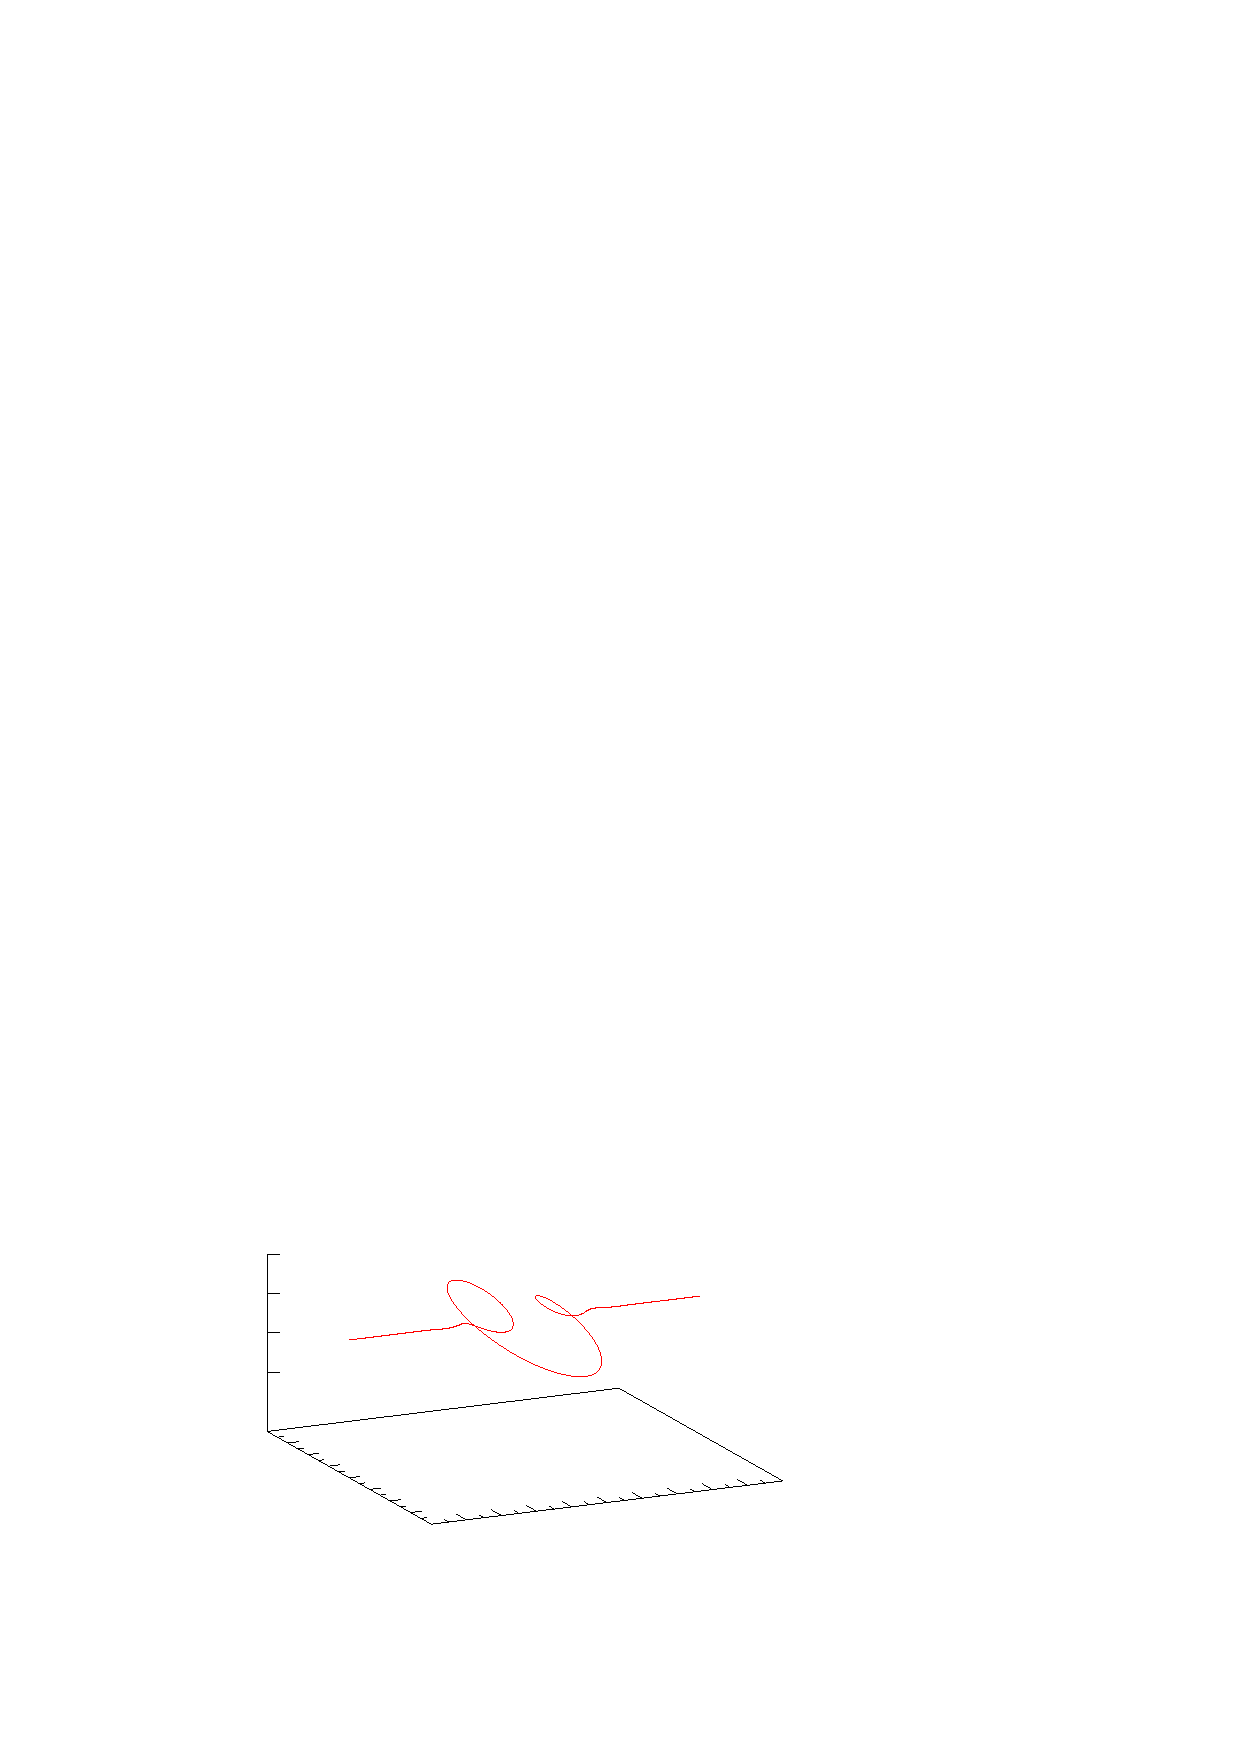
\includegraphics{Images/epslatex/lambda_P1_config}%
\end{picture}%
\begingroup
\setlength{\unitlength}{0.0200bp}%
\begin{picture}(18000,10800)(0,0)%
\put(6968,1667){\makebox(0,0){\strut{} 0}}%
\put(7812,1770){\makebox(0,0){\strut{} 0.2}}%
\put(8657,1874){\makebox(0,0){\strut{} 0.4}}%
\put(9500,1978){\makebox(0,0){\strut{} 0.6}}%
\put(10344,2082){\makebox(0,0){\strut{} 0.8}}%
\put(11188,2186){\makebox(0,0){\strut{} 1}}%
\put(12032,2290){\makebox(0,0){\strut{} 1.2}}%
\put(12876,2393){\makebox(0,0){\strut{} 1.4}}%
\put(13720,2497){\makebox(0,0){\strut{} 1.6}}%
\put(14565,2601){\makebox(0,0){\strut{} 1.8}}%
\put(15409,2705){\makebox(0,0){\strut{} 2}}%
\put(6499,1855){\makebox(0,0)[r]{\strut{}-2}}%
\put(6007,2133){\makebox(0,0)[r]{\strut{}-1.5}}%
\put(5515,2411){\makebox(0,0)[r]{\strut{}-1}}%
\put(5023,2689){\makebox(0,0)[r]{\strut{}-0.5}}%
\put(4531,2968){\makebox(0,0)[r]{\strut{} 0}}%
\put(4039,3246){\makebox(0,0)[r]{\strut{} 0.5}}%
\put(3547,3524){\makebox(0,0)[r]{\strut{} 1}}%
\put(3054,3803){\makebox(0,0)[r]{\strut{} 1.5}}%
\put(2562,4081){\makebox(0,0)[r]{\strut{} 2}}%
\put(2212,5560){\makebox(0,0)[r]{\strut{}-4}}%
\put(2212,6505){\makebox(0,0)[r]{\strut{}-2}}%
\put(2212,7450){\makebox(0,0)[r]{\strut{} 0}}%
\put(2212,8396){\makebox(0,0)[r]{\strut{} 2}}%
\put(2811,9460){\makebox(0,0){\strut{}$y$}}%
\put(11952,1878){\makebox(0,0){\strut{}$z$}}%
\put(2669,2769){\makebox(0,0){\strut{}$x$}}%
\put(2811,9460){\makebox(0,0){\strut{}$y$}}%
\end{picture}%
\endgroup
\endinput
 
\end{center}
\caption[Configuration of primary homoclinic]{\baselineskip=1.0\normalbaselineskip%
Configuration of primary homoclinic $P_{1}$ orbits in table~\ref{tab:rev0}.}
\label{fig:P1_config}
\end{figure} 
% 
\begin{figure}[h!tbp]
\begin{center}
\subfigure{ \input{Images/epslatex/R2_force_1.tex} \label{fig:R2_force_1} }
\subfigure{ %GNUPLOT: LaTeX picture with Postscript
\begin{picture}(0,0)%
\includegraphics{Images/epslatex/R2_force_2}%
\end{picture}%
\begingroup
\setlength{\unitlength}{0.0200bp}%
\begin{picture}(9900,5940)(0,0)%
\put(2475,1650){\makebox(0,0)[r]{\strut{}-0.06}}%
\put(2475,2273){\makebox(0,0)[r]{\strut{}-0.04}}%
\put(2475,2897){\makebox(0,0)[r]{\strut{}-0.02}}%
\put(2475,3520){\makebox(0,0)[r]{\strut{} 0}}%
\put(2475,4143){\makebox(0,0)[r]{\strut{} 0.02}}%
\put(2475,4767){\makebox(0,0)[r]{\strut{} 0.04}}%
\put(2475,5390){\makebox(0,0)[r]{\strut{} 0.06}}%
\put(2750,1100){\makebox(0,0){\strut{} 0}}%
\put(4015,1100){\makebox(0,0){\strut{} 0.2}}%
\put(5280,1100){\makebox(0,0){\strut{} 0.4}}%
\put(6545,1100){\makebox(0,0){\strut{} 0.6}}%
\put(7810,1100){\makebox(0,0){\strut{} 0.8}}%
\put(9075,1100){\makebox(0,0){\strut{} 1}}%
\put(550,3520){\rotatebox{90}{\makebox(0,0){\strut{}$f_{2}$}}}%
\put(5912,275){\makebox(0,0){\strut{}$s$}}%
\end{picture}%
\endgroup
\endinput
 \label{fig:R2_force_2} }
\end{center}
\caption[External force due to magnetic effects]{\baselineskip=1.0\normalbaselineskip%
External force due to magnetic effects for the $P_{1}$ orbits in table~\ref{tab:rev0}. Note that the external forces are reversible.} 
\label{fig:force}
\end{figure}
%
\begin{table}[h!t]
\caption[Shooting data for trimodal homoclinic orbits]{\baselineskip=1.0\normalbaselineskip%
Shooting data for some reversible trimodals homoclinic orbits when $\nu=1\slash3$, $m=1.90$, $\epsilon=0.1$ and $\lambda=0.1$.}
\begin{center}
\begin{tabular}{ccccc}
\hline
& & $\delta_{1}$ & $\delta_{2}$ & $\mathcal{T}$ \\ 
$R_{1}$ & $\left(P_{2},n,P_{2},n,P_{2}\right)$ & 1.449005 & 7.734693 & 101.7462 \\
& $\left(P_{3},n,P_{1},n,P_{4}\right)$ & 4.590598 & 7.734693 & 101.7462 \\
$R_{2}$ & $\left(P_{1},n,P_{4},n,P_{1}\right)$ & 0.5914260 & 6.264897 & 99.38831 \\
& $\left(P_{2},n,P_{3},n,P_{2}\right)$ & 3.7330187 & 6.264897 & 99.38831 \\
\hline
\end{tabular}
\label{tab:rev2}
\end{center}
\end{table}
%
\begin{figure}[h!tbp]
\begin{center}
\subfigure[][$P_{1},n,P_{1}$]{ \input{Images/epslatex/Bimodal_x_1.tex}\label{fig:bimodal_1} }
\subfigure[][$P_{1},n,P_{1}$]{ %GNUPLOT: LaTeX picture with Postscript
\begin{picture}(0,0)%
\includegraphics{Images/epslatex/Bimodal_x_2}%
\end{picture}%
\begingroup
\setlength{\unitlength}{0.0200bp}%
\begin{picture}(9900,6480)(0,0)%
\put(2200,1650){\makebox(0,0)[r]{\strut{}-0.6}}%
\put(2200,2261){\makebox(0,0)[r]{\strut{}-0.4}}%
\put(2200,2873){\makebox(0,0)[r]{\strut{}-0.2}}%
\put(2200,3484){\makebox(0,0)[r]{\strut{} 0}}%
\put(2200,4096){\makebox(0,0)[r]{\strut{} 0.2}}%
\put(2200,4707){\makebox(0,0)[r]{\strut{} 0.4}}%
\put(2200,5319){\makebox(0,0)[r]{\strut{} 0.6}}%
\put(2200,5930){\makebox(0,0)[r]{\strut{} 0.8}}%
\put(2475,1100){\makebox(0,0){\strut{} 0}}%
\put(3795,1100){\makebox(0,0){\strut{} 0.2}}%
\put(5115,1100){\makebox(0,0){\strut{} 0.4}}%
\put(6435,1100){\makebox(0,0){\strut{} 0.6}}%
\put(7755,1100){\makebox(0,0){\strut{} 0.8}}%
\put(9075,1100){\makebox(0,0){\strut{} 1}}%
\put(550,3790){\rotatebox{90}{\makebox(0,0){\strut{}$x_2$}}}%
\put(5775,275){\makebox(0,0){\strut{}$s$}}%
\end{picture}%
\endgroup
\endinput
\label{fig:bimodal_2} }
\subfigure[][$P_{2},n,P_{2},n,P_{2}$]{ \input{Images/epslatex/Trimodal_x_1.tex}\label{fig:trimodal_1} }
\subfigure[][$P_{2},n,P_{2},n,P_{2}$]{ \input{Images/epslatex/Trimodal_x_2.tex}\label{fig:trimodal_2} }
\end{center}
\caption[Force components of a bimodal homoclinic]{\baselineskip=1.0\normalbaselineskip%
Force component $x_{1}$ and $x_{2}$ of bimodal $P_{1},n,P_{2}$ from table~\ref{tab:rev1} shown in~\ref{fig:bimodal_1},~\ref{fig:bimodal_2} and for the trimodal $P_{2},n,P_{2},n,P_{2}$ in table~\ref{tab:rev2}.}
\label{fig:multimodals}
\end{figure} 
%
\par % Multimodals in anisotropic case
Multimodal solutions can be found in the anisotropic system, as shown in figure~\ref{fig:P1_anisotropic_full_quadmodal}, providing numerical evidence that, as in the Kirchhoff rod, anisotropy is an integrability breaking parameter for the linearly elastic, inextensible, unshearable rod in a uniform magnetic field. 
% 
\begin{figure}[h!tbp]
\begin{center}
%GNUPLOT: LaTeX picture with Postscript
\begin{picture}(0,0)%
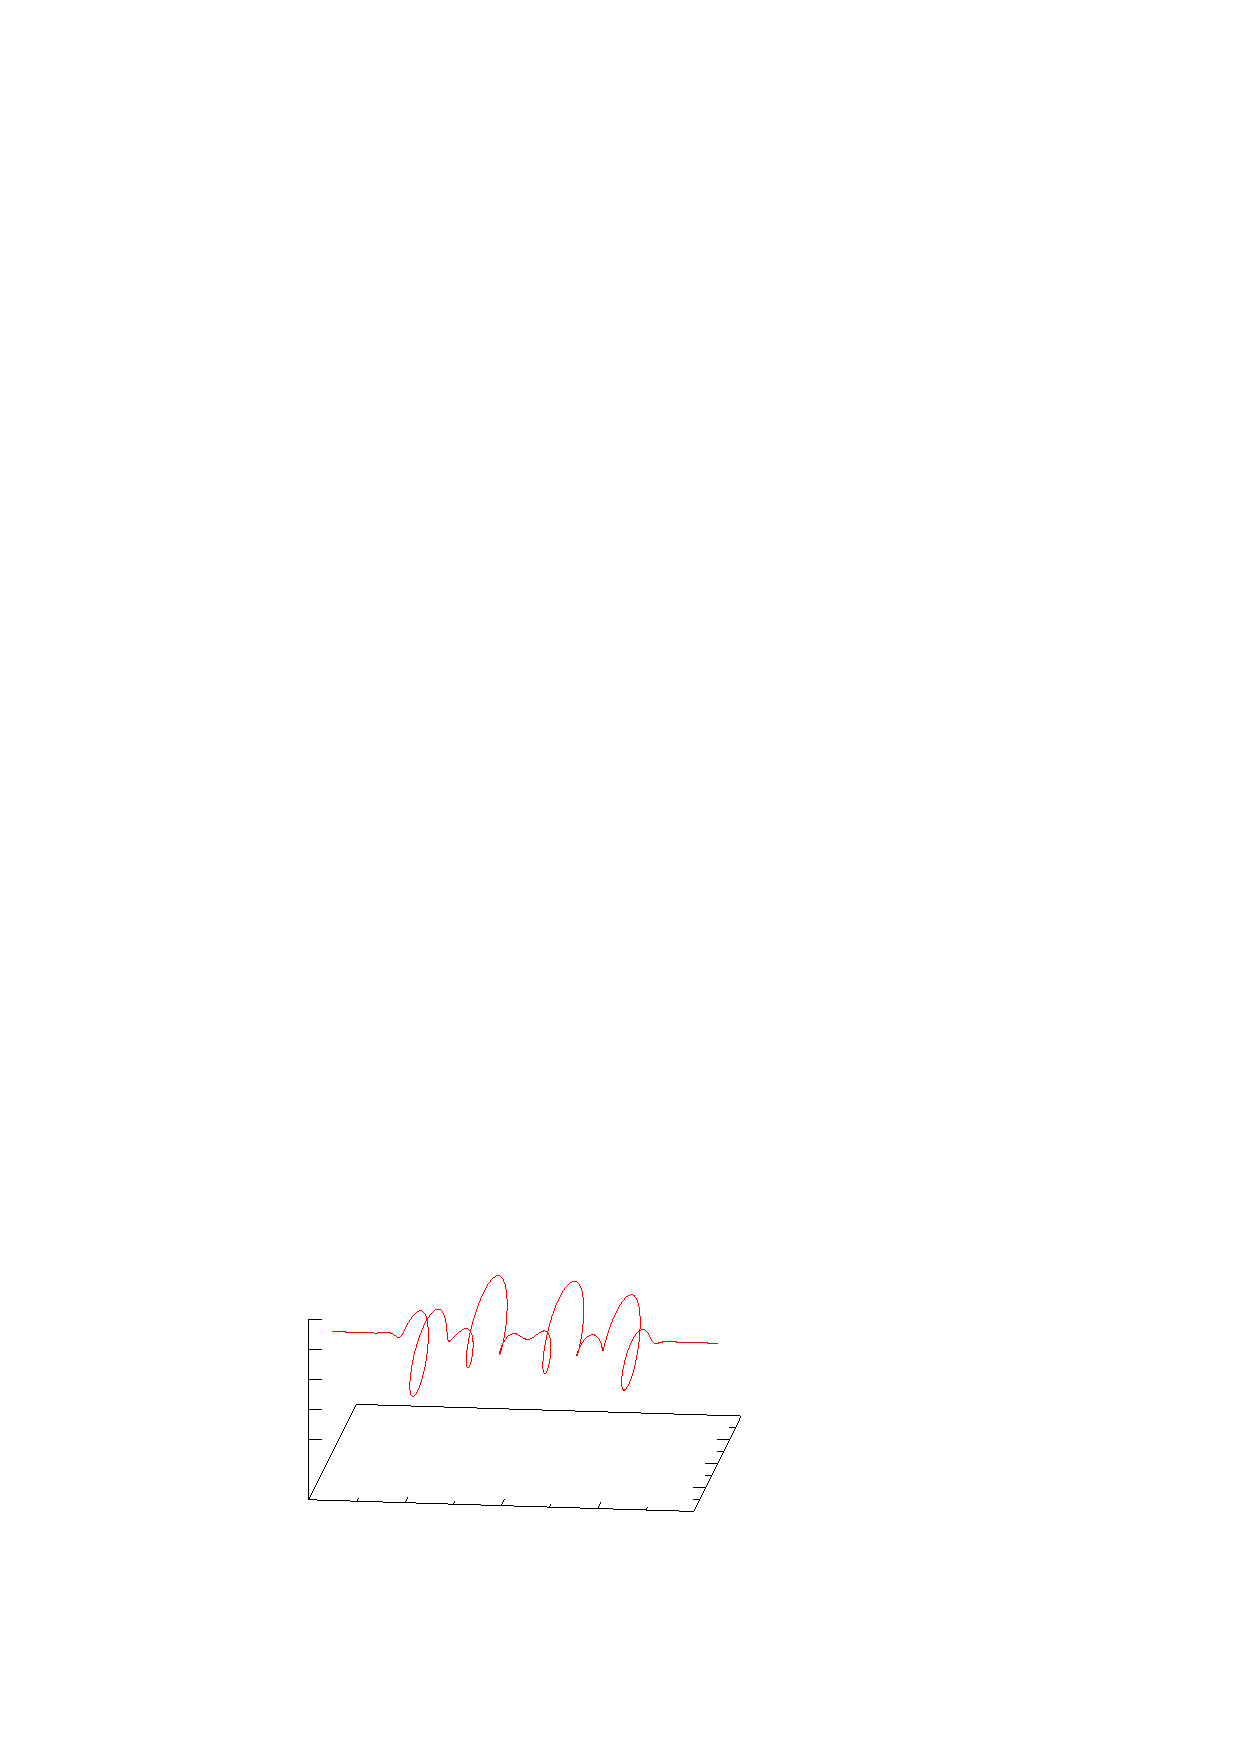
\includegraphics{Images/epslatex/P1_anisotropic_full_quadmodal}%
\end{picture}%
\begingroup
\setlength{\unitlength}{0.0200bp}%
\begin{picture}(18000,10800)(0,0)%
\put(3747,2246){\makebox(0,0){\strut{} 0}}%
\put(6058,2176){\makebox(0,0){\strut{} 0.5}}%
\put(8369,2106){\makebox(0,0){\strut{} 1}}%
\put(10680,2035){\makebox(0,0){\strut{} 1.5}}%
\put(12991,1965){\makebox(0,0){\strut{} 2}}%
\put(13327,2205){\makebox(0,0)[l]{\strut{}-2}}%
\put(13611,2777){\makebox(0,0)[l]{\strut{}-1}}%
\put(13895,3349){\makebox(0,0)[l]{\strut{} 0}}%
\put(14179,3922){\makebox(0,0)[l]{\strut{} 1}}%
\put(14462,4494){\makebox(0,0)[l]{\strut{} 2}}%
\put(3211,3948){\makebox(0,0)[r]{\strut{}-2}}%
\put(3211,4671){\makebox(0,0)[r]{\strut{}-1}}%
\put(3211,5394){\makebox(0,0)[r]{\strut{} 0}}%
\put(3211,6116){\makebox(0,0)[r]{\strut{} 1}}%
\put(3211,6839){\makebox(0,0)[r]{\strut{} 2}}%
\put(3810,7924){\makebox(0,0){\strut{}$x$}}%
\put(8149,1790){\makebox(0,0){\strut{}$z$}}%
\put(15933,3296){\makebox(0,0){\strut{}$y$}}%
\put(3810,7924){\makebox(0,0){\strut{}$x$}}%
\end{picture}%
\endgroup
\endinput
 
\end{center}
\caption[Multimodal configuration in the anisotropic rod in a magnetic field]{\baselineskip=1.0\normalbaselineskip%
A quadmodal with parameters are $\nu={1}\slash{3}$, $\lambda=0.01$, $m=1.70$ and $\rho=0.1$. When $\lambda=0.1$, $m=1.90$ the shooting parameters are given by $\delta_{1} = 5.2433$, $\delta_{2} = 2.1968$ and $\mathcal{T}=85.509$.} 
\label{fig:P1_anisotropic_full_quadmodal}
\end{figure}
% 
% \vspace*{2.0cm}
\section{Continuation} \label{sec:continuation}
%
\par % Projection boundary conditions 
In this section the continuation of configurations is performed using projection boundary conditions~\cite{Beyn90a,Beyn94} exploiting the exponential trichotomies the system possesses~\cite{Klaus03}. The method places solutions in the linearised flow which approximates the tangential flow about a equilibrium configuration. In this system the continuation of periodic-to-periodic homoclinic orbits is simplified~\cite{Champneys97d,Bai96a,Dieci04} by knowing the underlying periodic orbit~\eqref{eq:trivial}. Thus, projecting onto the two-dimensional centre and unstable (generalised) eigenspaces about the phase condition~\eqref{eq:phase} yields the four boundary conditions
%
\begin{subequations}
\label{eq:projection}
\begin{align}
L_{s}\left( \boldsymbol{x}\left(0\right) - \boldsymbol{p} \right) & = \boldsymbol{0}, \label{eq:stable_projection} \\
L_{c}\left( \boldsymbol{x}\left(0\right) - \boldsymbol{p} \right) & = \boldsymbol{0}. \label{eq:centre_projection}
\end{align}
\end{subequations}
% 
Applying the symmetric section boundary conditions, for $R_{1}$ as in~\eqref{eq:rhs}, yields the three boundary conditions
%
\begin{align}
x_{1}\left(1\right) = x_{4}\left(1\right) = x_{10}\left(1\right) & = 0. \label{eq:symmetric}
\end{align}
%
Finally, specifying the three Casimirs~\eqref{eq:nondim_casimirs} and the constraint fixing condition~\eqref{eq:nondim_constraint} gives four boundary conditions
%
\begin{align}
x_{3}\left(0\right) - 1 = x_{6}\left(0\right) - 1 & = x_{9}\left(0\right) = x_{10}\left(0\right) - 1 = 0. \label{eq:integral} 
\end{align}
%
The system~\eqref{eq:ge_full} with boundary conditions~\eqref{eq:projection},~\eqref{eq:symmetric} and~\eqref{eq:integral} is over-determined as there are eleven boundary conditions for a ten dimensional system. Specifically, the projection boundary conditions provide an extra condition, that is there are four boundary conditions determining a flow which can be determined by three (shooting) parameters. Thus, in order to make the problem well-posed the truncation length, $\mathcal{T}$, is allowed to vary along with the principal continuation parameter. %
%
\par % restriction on lambda
It should be noted that while there is no restriction on the sign of $\lambda$, when performing continuation an increase in $\lambda$ acts in the direction of the end load parameter $m$, while decreasing $\lambda$ acts against the load parameter. 
%
\par % Benefits of numerical schemes
Continuation was performed using \textsc{auto97}~\cite{Doedel98}. The continuation software uses Gaussian collocation, which is equivalent to a symplectic Runge-Kutta scheme. Symplectic Runge-Kutta methods exactly conserve the value of any integrals of the system that are quadratic functions of the phase variables~\cite{Channell90}.  Thus, from the Lax pair formulation, presented in \S\ref{sec:lax}, all the  conserved quantities are preserved by the numerical scheme. Note that the Kovalevskaya integral would not be preserved exactly as it is a quartic integral.
%
\par % End deflections
In order to visualise the rod configurations the postprocessed centreline conditions for $\boldsymbol{r}\left(s\right)=\left(x,y,z\right)$, which evolves according to~\eqref{eq:centreline}, are computed from
%
\begin{align}
\boldsymbol{r}\left(0\right) & = \boldsymbol{0}. \label{eq:centreline_ic}
\end{align}
%
Hence the (dimensionless) end-rotation and end-displacement can be calculated while continuing along solution branches of homoclinic orbits for the two parameters $\lambda$ and $\mathcal{T}$. The relative end-deflections represent the true buckling contributions due to the effect of loading by removing the trivial contributions from a unbuckled straight rod. Thus let the relative end-displacement, $\tilde{\mathcal{D}}$ and relative end-rotation $\tilde{\mathcal{R}}$ be given by
%
\begin{subequations}
\begin{align}
\tilde{\mathcal{D}} & = \left(1+\epsilon\right)\mathcal{T} - z\left(1\right), \\
\tilde{\mathcal{R}} & = \frac{\mathcal{R} - \left(1+\nu\right)\mathcal{T}}{2\pi} 
\end{align}
\end{subequations}
%
where 
%
\begin{equation}
\cos \mathcal{R} =\left< \boldsymbol{d}_{1}\left(1\right), \left(1,0,0\right)\right> \quad \mbox{and} \quad \sin \mathcal{R} =\left< \boldsymbol{d}_{1}\left(1\right), \left(0,1,0\right)\right>. \nonumber 
\end{equation}
%
\par
In many respects the end rotation can be thought of as a phase on the sphere defined by $\boldsymbol{r}$. For configurations which have zero first derivative at the end points, such as clamped and homoclinic configurations, the curves on the sphere can be considered to be closed and topological properties such as (open) link, (open) twist and (open) writhe can be related, in a consistent manner, to the phase on the sphere~\cite{Maggs01,Heijden07}. 
% The curves on the sphere are exactly closed on the sphere if the north pole is included, just as the curves in the phase plane illustrated in figure~\ref{fig:super} are closed if the origin is included, cf. remark~\ref{rem:homoclinic}. 
% 
% \begin{figure}[h!tbp]
% \begin{center}
% \input{Images/epslatex/sphere.tex} 
% \end{center}
% \caption[]{\baselineskip=1.0\normalbaselineskip } 
% \label{fig:sphere}
% \end{figure}
% % 
% Then $\mathcal{R}$ is the (open) link, $\left(1+\nu\right)\mathcal{T}$ is the local twist and $\mathcal{R}$ is the writhe of the rod in the celebrated C$\breve{\mathrm{a}}$lug$\breve{\mathrm{a}}$reanu formula~\cite{Langer84}.
%
% \par
% When the end-rotation and end-deflection are zero the rod is a straight rod, hence configurations exists on a one-dimensional Liouville tori. It is an open question whether a relationship, either a homomorphism or an isomorphism, exists relating the analytical expressions of the end-deflections to the angular coordinates of a set of action-angle variables exists. Phase on the torus? 
%
\section{Bifurcation} \label{sec:bifurcation}
% 
\par % Intro
Having established bifurcation structure for homoclinic orbits in the four-dimensional strictly hyperbolic case in~\S\ref{sec:conseq}, in this section the bifurcation behaviour of primary homoclinics in the homoclinic-to-periodic case is investigated. 
% 
\par % New bifurcation
Due to the coupling between the force and moments and the magnetic field, the straight twisted rod is a periodic solution~\eqref{eq:trivial} and hence the bifurcation structure of the system is different from the classical Kirchhoff rod. The rod now buckles in a twice generalised Hopf bifurcation: firstly by being Hamiltonian and secondly by being about a periodic orbit. Thus, the bifurcation may be described as Hamiltonian-Hopf bifurcation about a periodic solution, a Hamiltonian-\u{S}il'nikov bifurcation or alternately as a Hamiltonian Naimark-Sacker bifurcation. 
%
\par
Subcritical bifurcations in arbitrarily long structures are associated with localised buckling, as is the case for the Kirchhoff rod, whereas supercritical bifurcations produce periodic responses. The localisation-delocalisation-localisation behaviour observed is characteristic of the interplay between the localisation associated with a homoclinic orbit and delocalisation associated with periodicity.
% 
\par % Primaries
Load-deflection diagrams of primary homoclinics for continuation in $\lambda$ are presented in figure~\ref{fig:lambda}. Interestingly, regions are found where homoclinic configurations actually buckle with $\lambda$ decreasing as well as increasing.  From the analysis of the Floquet multipliers, the codimension-two point delineates between primary homoclinic configurations which can buckle at two values $\lambda_{+}$, $\lambda_{-}$, one value, $\lambda_{c}$ or which do not buckle at all. The figure~\ref{fig:lambda} illustrates all three possible situations.  From subfigure~\ref{fig:buckling_m_1.9000} it can be seen that localised solutions with $m=1.90$ and $\epsilon=0.1$ buckle from the right at $\lambda_{+}=0.076370$ and from the left at $\lambda_{-}=0.087626$. The buckling values predicted through the Floquet multipliers are $\lambda_{+}=0.07648203$ and $\lambda_{+}=0.08756156$. Rod configurations are quantitatively the same whether the bifurcation values are approached from either the left or the right. 
%
\par % Interpretation
Figures~\ref{fig:lambda} and~\ref{fig:m_buckling} illustrates that the effect of the magnetic field on the configurations produces two distinct scenarios depending on the value of end loading $m$ in relation to the codimension-two point $m_{c}$. If $m<m_{c}$ then localising-buckling occurs as illustrated in subfigure~\ref{fig:buckling_m_1.9000} or if $m>m_{c}$ then localising-delocalising-localising behaviour occurs as illustrated by subfigure~\ref{fig:buckling_m_1.8100}. Quantitively, the localising-delocalising-localising behaviour has been seen before under a variety of guises as the softening-hardening-softening response for a rod is constrained to lie on a cylinder~\cite{Heijden02b} and destabilisation-restabilistion behaviour of a rod on an elastic foundation near to the Maxwell load~\cite{Hunt00}. It should be stressed that this situation is qualitatively different as the primary homoclinic orbits do not gain extra modes as the perturbed manifold intersects the symmetric section.
%
\begin{figure}[h!tbp]
\begin{center}
\subfigure[][$m=1.9 > m_{c}$]{
\input{Images/epslatex/R1_lambda_m_1.9000_R.tex}
%GNUPLOT: LaTeX picture with Postscript
\begin{picture}(0,0)%
\includegraphics{Images/epslatex/R1_lambda_m_1.9000_D.eps}%
\end{picture}%
\begingroup
\setlength{\unitlength}{0.0200bp}%
\begin{picture}(9900,6480)(0,0)%
\put(1925,1650){\makebox(0,0)[r]{\strut{} 0}}%
\put(1925,2506){\makebox(0,0)[r]{\strut{} 2}}%
\put(1925,3362){\makebox(0,0)[r]{\strut{} 4}}%
\put(1925,4218){\makebox(0,0)[r]{\strut{} 6}}%
\put(1925,5074){\makebox(0,0)[r]{\strut{} 8}}%
\put(1925,5930){\makebox(0,0)[r]{\strut{} 10}}%
\put(2200,1100){\makebox(0,0){\strut{} 0}}%
\put(3575,1100){\makebox(0,0){\strut{} 0.025}}%
\put(4950,1100){\makebox(0,0){\strut{} 0.05}}%
\put(6325,1100){\makebox(0,0){\strut{} 0.075}}%
\put(7700,1100){\makebox(0,0){\strut{} 0.1}}%
\put(9075,1100){\makebox(0,0){\strut{} 0.125}}%
\put(550,3790){\rotatebox{90}{\makebox(0,0){\strut{}$\tilde{\mathcal{D}}$}}}%
\put(5637,275){\makebox(0,0){\strut{}$\lambda$}}%
\end{picture}%
\endgroup
\endinput
\label{fig:m_1.9000} }
\subfigure[][$m=1.8211 = m_{c}$]{
%GNUPLOT: LaTeX picture with Postscript
\begin{picture}(0,0)%
\includegraphics{Images/epslatex/R1_lambda_m_1.8211_R.eps}%
\end{picture}%
\begingroup
\setlength{\unitlength}{0.0200bp}%
\begin{picture}(9900,6480)(0,0)%
\put(2475,1650){\makebox(0,0)[r]{\strut{} 0}}%
\put(2475,2126){\makebox(0,0)[r]{\strut{} 0.05}}%
\put(2475,2601){\makebox(0,0)[r]{\strut{} 0.1}}%
\put(2475,3077){\makebox(0,0)[r]{\strut{} 0.15}}%
\put(2475,3552){\makebox(0,0)[r]{\strut{} 0.2}}%
\put(2475,4028){\makebox(0,0)[r]{\strut{} 0.25}}%
\put(2475,4503){\makebox(0,0)[r]{\strut{} 0.3}}%
\put(2475,4979){\makebox(0,0)[r]{\strut{} 0.35}}%
\put(2475,5454){\makebox(0,0)[r]{\strut{} 0.4}}%
\put(2475,5930){\makebox(0,0)[r]{\strut{} 0.45}}%
\put(2750,1100){\makebox(0,0){\strut{} 0}}%
\put(4015,1100){\makebox(0,0){\strut{} 0.025}}%
\put(5280,1100){\makebox(0,0){\strut{} 0.05}}%
\put(6545,1100){\makebox(0,0){\strut{} 0.075}}%
\put(7810,1100){\makebox(0,0){\strut{} 0.1}}%
\put(9075,1100){\makebox(0,0){\strut{} 0.125}}%
\put(550,3790){\rotatebox{90}{\makebox(0,0){\strut{}$\tilde{\mathcal{R}}$}}}%
\put(5912,275){\makebox(0,0){\strut{}$\lambda$}}%
\end{picture}%
\endgroup
\endinput

\input{Images/epslatex/R1_lambda_m_1.8211_D.tex}\label{fig:m_1.8211} }
\subfigure[][$m=1.81 < m_{c}$]{
\input{Images/epslatex/R1_lambda_m_1.8100_R.tex}
\input{Images/epslatex/R1_lambda_m_1.8100_D.tex}\label{fig:m_1.8100} }
\caption[Load-deflection curves for a primary homoclinic about the codimension-two point]{\baselineskip=1.0\normalbaselineskip%
Load-displacement diagrams for $\lambda$, when $m$ is above, equal and below the codimension-two point $m_{c}$.}
\label{fig:lambda}
\end{center}
\end{figure}
%
\begin{figure}[h!tbp]
\begin{center}
\subfigure[][$m=1.90 > m_{c}$]{\input{Images/epslatex/buckling_m_1.9000.tex}\label{fig:buckling_m_1.9000} }
\subfigure[][$m=1.81 < m_{c}$]{%GNUPLOT: LaTeX picture with Postscript
\begin{picture}(0,0)%
\includegraphics{Images/epslatex/buckling_m_1.8100.eps}%
\end{picture}%
\begingroup
\setlength{\unitlength}{0.0200bp}%
\begin{picture}(18000,10800)(0,0)%
\put(1925,1650){\makebox(0,0)[r]{\strut{} 0}}%
\put(1925,3214){\makebox(0,0)[r]{\strut{} 2}}%
\put(1925,4777){\makebox(0,0)[r]{\strut{} 4}}%
\put(1925,6341){\makebox(0,0)[r]{\strut{} 6}}%
\put(1925,7905){\makebox(0,0)[r]{\strut{} 8}}%
\put(1925,9468){\makebox(0,0)[r]{\strut{} 10}}%
\put(2200,1100){\makebox(0,0){\strut{} 0}}%
\put(4419,1100){\makebox(0,0){\strut{} 0.02}}%
\put(6637,1100){\makebox(0,0){\strut{} 0.04}}%
\put(8856,1100){\makebox(0,0){\strut{} 0.06}}%
\put(11074,1100){\makebox(0,0){\strut{} 0.08}}%
\put(13293,1100){\makebox(0,0){\strut{} 0.1}}%
\put(15511,1100){\makebox(0,0){\strut{} 0.12}}%
\put(550,5950){\rotatebox{90}{\makebox(0,0){\strut{}$\tilde{\mathcal{D}}$}}}%
\put(9687,275){\makebox(0,0){\strut{}$\lambda$}}%
\end{picture}%
\endgroup
\endinput
\label{fig:buckling_m_1.8100} }
\caption[Localised buckling above and below the codimension-two point]{\baselineskip=1.0\normalbaselineskip% 
Subfigure~\ref{fig:buckling_m_1.9000} shows buckling for both $\lambda_{-}=0.087626$ or $\lambda_{+}=0.07637$ above the codimension-two point when $m=1.90$. Subfigure~\ref{fig:buckling_m_1.8100} shows the localisation-delocalisation-localisation behaviour below the codimension-two point at $m=1.81$. Again, in both subfigures $\nu=1\slash{3}$ and $\epsilon=0.1$.}
\label{fig:m_buckling}
\end{center}
\end{figure}
% 
% \vspace*{-20pt}
\par % Far beyond
For values of $m$ far below the codimension-two point the load-deflection diagrams do not always behave as those near or greater than the codimension-two point $m_{c}$.  As can be seen from figure~\ref{fig:m_1.7398} for $m=1.7398$ and $\epsilon=0.1$; initially as $\lambda$ increases so $\tilde{\mathcal{R}}$ decreases while $\tilde{\mathcal{D}}$ increases, in contrast to the behaviour in subfigure~\ref{fig:m_1.8100}. It seems that for the end rotation the critical value of $\lambda$ corresponds to a minima, for the end deflection it corresponds to a point of inflection. Indeed, given the bifurcation diagrams in figure~\ref{fig:m_1.7398} one should expect that there exists a critical $m$ in the interval $1.7398<m<1.81$ at which the end-deflection diagram is seemingly constant until $\lambda$ is sufficiently large and the end-deflection increases. Quantitatively, in this regime localisation dominates and the rod configurations are all alike. Thus, for primary homoclinics continued in $\lambda$ the codimension-two point delineates between localisation-delocalisation-buckling and localisation-delocalisation-localisation but further away from the codimension-two point the influence of the delocalisation diminishes and localisation dominates. It should be noted that linear analysis from the Floquet multipliers does not shed any light on subtle changes in the rod configurations.
% 
\begin{figure}[h!tbp]
\begin{center}
\subfigure{%GNUPLOT: LaTeX picture with Postscript
\begin{picture}(0,0)%
\includegraphics{Images/epslatex/R1_lambda_m_1.7398_R.eps}%
\end{picture}%
\begingroup
\setlength{\unitlength}{0.0200bp}%
\begin{picture}(9900,6480)(0,0)%
\put(2750,1650){\makebox(0,0)[r]{\strut{} 0.25}}%
\put(2750,2506){\makebox(0,0)[r]{\strut{} 0.275}}%
\put(2750,3362){\makebox(0,0)[r]{\strut{} 0.3}}%
\put(2750,4218){\makebox(0,0)[r]{\strut{} 0.325}}%
\put(2750,5074){\makebox(0,0)[r]{\strut{} 0.35}}%
\put(2750,5930){\makebox(0,0)[r]{\strut{} 0.375}}%
\put(3025,1100){\makebox(0,0){\strut{} 0}}%
\put(4235,1100){\makebox(0,0){\strut{} 0.025}}%
\put(5445,1100){\makebox(0,0){\strut{} 0.05}}%
\put(6655,1100){\makebox(0,0){\strut{} 0.075}}%
\put(7865,1100){\makebox(0,0){\strut{} 0.1}}%
\put(9075,1100){\makebox(0,0){\strut{} 0.125}}%
\put(550,3790){\rotatebox{90}{\makebox(0,0){\strut{}$\tilde{\mathcal{R}}$}}}%
\put(6050,275){\makebox(0,0){\strut{}$\lambda$}}%
\end{picture}%
\endgroup
\endinput
\label{fig:m_1.7398_R} }
\subfigure{%GNUPLOT: LaTeX picture with Postscript
\begin{picture}(0,0)%
\includegraphics{Images/epslatex/R1_lambda_m_1.7398_D.eps}%
\end{picture}%
\begingroup
\setlength{\unitlength}{0.0200bp}%
\begin{picture}(9900,6480)(0,0)%
\put(2200,1650){\makebox(0,0)[r]{\strut{} 4}}%
\put(2200,2363){\makebox(0,0)[r]{\strut{} 4.5}}%
\put(2200,3077){\makebox(0,0)[r]{\strut{} 5}}%
\put(2200,3790){\makebox(0,0)[r]{\strut{} 5.5}}%
\put(2200,4503){\makebox(0,0)[r]{\strut{} 6}}%
\put(2200,5217){\makebox(0,0)[r]{\strut{} 6.5}}%
\put(2200,5930){\makebox(0,0)[r]{\strut{} 7}}%
\put(2475,1100){\makebox(0,0){\strut{} 0}}%
\put(3795,1100){\makebox(0,0){\strut{} 0.025}}%
\put(5115,1100){\makebox(0,0){\strut{} 0.05}}%
\put(6435,1100){\makebox(0,0){\strut{} 0.075}}%
\put(7755,1100){\makebox(0,0){\strut{} 0.1}}%
\put(9075,1100){\makebox(0,0){\strut{} 0.125}}%
\put(550,3790){\rotatebox{90}{\makebox(0,0){\strut{}$\tilde{\mathcal{D}}$}}}%
\put(5775,275){\makebox(0,0){\strut{}$\lambda$}}%
\end{picture}%
\endgroup
\endinput
\label{fig:m_1.7398_D} }
\caption[Load-deflection curves for a primary homoclinic far below the codimension-two point]{\baselineskip=1.0\normalbaselineskip%
Load-deflection diagrams for $\lambda$ far below the codimension two point at $m=1.7398<<m_{c}$. The critical value of $\lambda$ is given by $\lambda=0.1128947$ although there seems to be little quantitative difference between solutions near this value.}
\label{fig:m_1.7398}
\end{center}
\end{figure}
%
\par % Schematic diagrams twice bifurcation
As has been mentioned the bifurcation is a twice generalised Hopf bifurcation. The Hamiltonian structure means that the Floquet multipliers will appear in conjugate pairs and the periodicity means that a pair of multipliers will always be on the unit circle.  Schematic diagrams in figures~\ref{fig:bif_diagram} and~\ref{fig:bif_diagram_codim} illustrate the observed bifurcation mechanism in terms of the Floquet multipliers. In the generic case, starting from $\lambda=0$, with $m>m_{c}$, while the centre Floquet multipliers, $\mu^{c}$, move around the unit circle, the stable and unstable Floquet multipliers, $\mu^{s,u}$, collide on the unit circle at $\lambda=\lambda_{-}$. The multipliers then split and move around the unit circle in opposite directions before one pair collides with the centre multipliers at $\lambda_{+}$. The multipliers then split again to become the stable and unstable multipliers. As can be inferred from figure~\ref{fig:m_buckling} the process can be described in reverse as $\lambda$ decreases.
%
\par % Schematic diagrams once bifurcation
When $m=m_{c}$ the centre Floquet multipliers move around the unit centre which sufficient speed so that at $\lambda=\lambda_{c}$ all the Floquet multipliers collide on the unit circle. Thus, the codimension-two point is a generalised Hopf-Hopf bifurcation point. One pair remains on, one pair are within, and one the pair are outside of the unit circle, as with the original spectrum as $\lambda=0$. At the codimension-two point it is not possible to say how the Floquet multipliers behave without nonlinear normal form analysis. It could be the case that two of the pairs of multipliers split on the unit circle while the remaining pair pass on the unit circle, however it is possible that the bifurcation at this singular point is qualitatively different from previous bifurcations. 
%
\par
On analysis of the Floquet multipliers it is clear that the six-dimensions is the minimal system at which two distinct Hamiltonian-Hopf bifurcations can occur and that two multipliers must be on the unit circle or imaginary axis. It is unfortunate thus due to the underlying periodicity of the monodromy matrix that no analytical expressions for the codimension-two point can be found. The two loading parameters `unfold' the dynamics; in a sense $\lambda$ determines the Hamiltonian-Hopf bifurcations and $m$ determines the distance between the bifurcations and that at $\left(\lambda_{c},m_{c}\right)$ the two bifurcations occur simultaneously. Thus normal form analysis would be six-dimensional and have two unfolding parameters. As shall be seen later, the double Hamiltonian-Hopf bifurcation provides an organising centre for the bifurcation set of primary and multimodal homoclinics. 
%
\begin{figure}[h!tbp]%
\begin{center}%
\setlength{\unitlength}{1.0cm}%
\begin{picture}(15,4.5)(0,0.5)%
\linethickness{1pt}%
\put(0.5,2.5){\vector(1,0){2}}%
\put(1.5,1.5){\vector(0,1){2}}%
\put(1.5,2.5){\circle{10}}%
\put(2.225,2.5){\circle*{0.1}}%
\put(1.325,2.8){\circle{0.1}}%
\put(1.325,2.2){\circle{0.1}}%
\put(0.995,3.3){\circle{0.1}}%
\put(0.995,1.7){\circle{0.1}}%
\put(1.5,1.0){ \makebox(0,0)[c]{ \mbox{ {\small $\left(i\right)$} } } }%
\put(0.7,4.0){ \makebox(0,0)[l]{ \mbox{ {\small $\lambda = 0$} } } }%
\put(3.5,2.5){\vector(1,0){2}}%
\put(4.5,1.5){\vector(0,1){2}}%
\put(4.5,2.5){\circle{10}}%
\put(5.1,2.900){\circle{0.1}}%
\put(5.1,2.100){\circle{0.1}}%
\put(4.,3.0){\circle*{0.1}}%
\put(4.,2.0){\circle*{0.1}}%
\put(4.5,1.0){ \makebox(0,0)[c]{ \mbox{ {\small $\left(ii\right)$} } } }%
\put(3.7,4.0){ \makebox(0,0)[l]{ \mbox{ {\small $\lambda = \lambda_{-}$} } } }%
\put(6.5,2.5){\vector(1,0){2}}%
\put(7.5,1.5){\vector(0,1){2}}%
\put(7.5,2.5){\circle{10}}%
\put(7.8,3.15){\circle{0.1}}%
\put(7.8,1.85){\circle{0.1}}%
\put(6.85,2.8){\circle{0.1}}%
\put(6.85,2.2){\circle{0.1}}%
\put(7.4,3.200){\circle{0.1}}%
\put(7.4,1.800){\circle{0.1}}%
\put(7.5,1.0){ \makebox(0,0)[c]{ \mbox{ {\small $\left(iii\right)$} } } }%
\put(6.15,4.0){ \makebox(0,0)[l]{ \mbox{ {\small $\lambda_{-} < \lambda < \lambda_{+}$} } } }%
\put(9.5,2.5){\vector(1,0){2}}%
\put(10.5,1.5){\vector(0,1){2}}%
\put(10.5,2.5){\circle{10}}%
\put(10.85,3.1){\circle*{0.1}}%
\put(10.85,1.9){\circle*{0.1}}%
\put(9.85,2.75){\circle{0.1}}%
\put(9.85,2.25){\circle{0.1}}%
\put(10.5,1.0){ \makebox(0,0)[c]{ \mbox{ {\small $\left(iv\right)$} } } }%
\put(9.7,4.0){ \makebox(0,0)[l]{ \mbox{ {\small $\lambda = \lambda_{+}$} } } }%
\put(12.5,2.5){\vector(1,0){2}}%
\put(13.5,1.5){\vector(0,1){2}}%
\put(13.5,2.5){\circle{10}}%
\put(12.825,2.70){\circle{0.1}}%
\put(12.825,2.30){\circle{0.1}}%
\put(14.550,3.175){\circle{0.1}}%
\put(14.550,1.825){\circle{0.1}}%
\put(13.675,2.16){\circle{0.1}}%
\put(13.675,2.85){\circle{0.1}}%
\put(13.5,1.0){ \makebox(0,0)[c]{ \mbox{ {\small $\left(v\right)$} } } }%
\put(12.7,4.0){ \makebox(0,0)[l]{ \mbox{ {\small $\lambda > \lambda_{+}$} } } }%
\end{picture}%
\caption[Schematic diagram of the twice generalised Hopf bifurcation in the generic case]{\baselineskip=1.0\normalbaselineskip%
Schematic diagram of the twice generalised Hopf bifurcation in the generic case when $m>m_{c}$.}%
\label{fig:bif_diagram}% 
\end{center}%
\end{figure}%
% 
\begin{figure}[h!tbp]%
\begin{center}%
\setlength{\unitlength}{1.0cm}%
\begin{picture}(15,4.5)(0,0.5)%
\linethickness{1pt}%
\put(0.5,2.5){\vector(1,0){2}}%
\put(1.5,1.5){\vector(0,1){2}}%
\put(1.5,2.5){\circle{10}}%
\put(2.225,2.5){\circle*{0.1}}%
\put(1.325,2.8){\circle{0.1}}%
\put(1.325,2.2){\circle{0.1}}%
\put(0.995,3.3){\circle{0.1}}%
\put(0.995,1.7){\circle{0.1}}%
\put(1.5,1.0){ \makebox(0,0)[c]{ \mbox{ {\small $\left(i\right)$} } } }%
\put(0.7,4.0){ \makebox(0,0)[l]{ \mbox{ {\small $\lambda = 0$} } } }%
\put(3.5,2.5){\vector(1,0){2}}%
\put(4.5,1.5){\vector(0,1){2}}%
\put(4.5,2.5){\circle{10}}%
\put(4.1,2.10){\circle{0.1}}%
\put(4.1,2.90){\circle{0.1}}%
\put(3.95,3.10){\circle{0.1}}%
\put(3.95,1.90){\circle{0.1}}%
\put(4.25,3.1725){\circle{0.1}}%
\put(4.25,1.835){\circle{0.1}}%
\put(4.5,1.0){ \makebox(0,0)[c]{ \mbox{ {\small $\left(ii\right)$} } } }%
\put(3.7,4.0){ \makebox(0,0)[l]{ \mbox{ {\small $\lambda < \lambda_{c}$} } } }%
\put(6.5,2.5){\vector(1,0){2}}%
\put(7.5,1.5){\vector(0,1){2}}%
\put(7.5,2.5){\circle{10}}%
\put(7,3){\circle*{0.1}}%
\put(7,2){\circle*{0.1}}%
\put(7,3){\circle{0.175}}%
\put(7,2){\circle{0.175}}%
\put(7.5,1.0){ \makebox(0,0)[c]{ \mbox{ {\small $\left(iii\right)$} } } }%
\put(6.7,4.0){ \makebox(0,0)[l]{ \mbox{ {\small $\lambda = \lambda_{c}$} } } }%
\put(9.5,2.5){\vector(1,0){2}}%
\put(10.5,1.5){\vector(0,1){2}}%
\put(10.5,2.5){\circle{10}}%
\put(10.1,2.10){\circle{0.1}}%
\put(10.1,2.90){\circle{0.1}}%
\put(9.95,3.10){\circle{0.1}}%
\put(9.95,1.95){\circle{0.1}}%
\put(9.9,2.85){\circle{0.1}}%
\put(9.9,2.15){\circle{0.1}}%
\put(10.5,1.0){ \makebox(0,0)[c]{ \mbox{ {\small $\left(iv\right)$} }  } }%
\put(9.7,4.0){ \makebox(0,0)[l]{ \mbox{ {\small $\lambda > \lambda_{c}$} } } }%
\put(12.5,2.5){\vector(1,0){2}}%
\put(13.5,1.5){\vector(0,1){2}}%
\put(13.5,2.5){\circle{10}}%
\put(12.825,2.70){\circle{0.1}}%
\put(12.825,2.30){\circle{0.1}}%
\put(12.450,3.175){\circle{0.1}}%
\put(12.450,1.825){\circle{0.1}}%
\put(13.325,2.16){\circle{0.1}}%
\put(13.325,2.85){\circle{0.1}}%
\put(13.5,1.0){ \makebox(0,0)[c]{ \mbox{ {\small $\left(v\right)$} } } }%
\put(12.7,4.0){ \makebox(0,0)[l]{ \mbox{ {\small $\lambda \gg \lambda_{c}$} } } }%
\end{picture}%
\caption[Schematic diagram of the twice generalised Hopf bifurcation at the codimension-two point]{\baselineskip=1.0\normalbaselineskip%
Schematic diagram of the twice generalised Hopf bifurcation at the codimension-two point $m=m_{c}$.}%
\label{fig:bif_diagram_codim}% 
\end{center}%
\end{figure}%
% 
% \par % Possible normal form
% The bifurcation could be analysed through a normal form analysis using a Poincar\'e map, as outlined in~\cite[{\S{7.4.3}}]{Seydel94}. Let a Poincar\'e section, normal to the flow be $\Sigma$, then all iterates of the map will be bounded by a closed curve $U \in \Sigma$. Thus, all iterates of the map are bounded by a `drift-ring' and all orbits by a `torus-like' object.  As the bifurcation parameter reaches a critical value, the diameter of the torus and the area of the drift ring tend to zero as the configurations tend to straight, twisted rods. 
% 
\par % End loading
For comparison the effect of a constant magnetic field on the buckling of a rod due to end loading $m$ is illustrated in figure~\ref{fig:m} when $\lambda < \lambda_{c}$. It is observed that the presence of the magnetic field leads to an significant decrease in the end displacements and the buckling loads.
%
\begin{figure}[h!tbp] 
\begin{center}
\subfigure{%GNUPLOT: LaTeX picture with Postscript
\begin{picture}(0,0)%
\includegraphics{Images/epslatex/R1_m_lambda_R}%
\end{picture}%
\begingroup
\setlength{\unitlength}{0.0200bp}%
\begin{picture}(9900,6480)(0,0)%
\put(2200,1650){\makebox(0,0)[r]{\strut{} 0}}%
\put(2200,2506){\makebox(0,0)[r]{\strut{} 0.2}}%
\put(2200,3362){\makebox(0,0)[r]{\strut{} 0.4}}%
\put(2200,4218){\makebox(0,0)[r]{\strut{} 0.6}}%
\put(2200,5074){\makebox(0,0)[r]{\strut{} 0.8}}%
\put(2200,5930){\makebox(0,0)[r]{\strut{} 1}}%
\put(2475,1100){\makebox(0,0){\strut{} 0}}%
\put(3795,1100){\makebox(0,0){\strut{} 0.5}}%
\put(5115,1100){\makebox(0,0){\strut{} 1}}%
\put(6435,1100){\makebox(0,0){\strut{} 1.5}}%
\put(7755,1100){\makebox(0,0){\strut{} 2}}%
\put(9075,1100){\makebox(0,0){\strut{} 2.5}}%
\put(550,3790){\rotatebox{90}{\makebox(0,0){\strut{}$\tilde{\mathcal{R}}$}}}%
\put(5775,275){\makebox(0,0){\strut{}$m$}}%
\end{picture}%
\endgroup
\endinput
\label{fig:m_R} }
\subfigure{%GNUPLOT: LaTeX picture with Postscript
\begin{picture}(0,0)%
\includegraphics{Images/epslatex/R1_m_lambda_D}%
\end{picture}%
\begingroup
\setlength{\unitlength}{0.0200bp}%
\begin{picture}(9900,6480)(0,0)%
\put(1650,1650){\makebox(0,0)[r]{\strut{} 0}}%
\put(1650,2506){\makebox(0,0)[r]{\strut{} 1}}%
\put(1650,3362){\makebox(0,0)[r]{\strut{} 2}}%
\put(1650,4218){\makebox(0,0)[r]{\strut{} 3}}%
\put(1650,5074){\makebox(0,0)[r]{\strut{} 4}}%
\put(1650,5930){\makebox(0,0)[r]{\strut{} 5}}%
\put(1925,1100){\makebox(0,0){\strut{} 0}}%
\put(3355,1100){\makebox(0,0){\strut{} 0.5}}%
\put(4785,1100){\makebox(0,0){\strut{} 1}}%
\put(6215,1100){\makebox(0,0){\strut{} 1.5}}%
\put(7645,1100){\makebox(0,0){\strut{} 2}}%
\put(9075,1100){\makebox(0,0){\strut{} 2.5}}%
\put(550,3790){\rotatebox{90}{\makebox(0,0){\strut{}$\tilde{\mathcal{D}}$}}}%
\put(5500,275){\makebox(0,0){\strut{}$m$}}%
\end{picture}%
\endgroup
\endinput
\label{fig:m_D} }
\end{center}
\caption[Load-deflection curves for a primary homoclinic under end loading]{\baselineskip=1.0\normalbaselineskip%
Load-deflection diagrams for primary homoclinics when $\nu=1\slash3$, $\epsilon=0.1$. The blue-dashed line corresponds to $\lambda=0.01$ and buckles at $m=2.074667$ and the solid red line corresponds to $\lambda=0.05$ and this buckles at $m=1.975754$.}
\label{fig:m}
\end{figure}
%
\par % Anisotropy
Similarly, the effect of the magnetic field on the buckling of the rod due to anisotropy is illustrated in figure~\ref{fig:rho}. Once again the presence of the magnetic field leads to a decrease in the buckling value and the end displacements. It should be noted that the bifurcation observed is also a Hamiltonian-Hopf bifurcation about a periodic solution. It is not yet known whether there exist a codimension-two point $\left(\rho_{c},\lambda_{c}\right)$ which delineates between weakly anisotropic rods (which buckle in Hamiltonian-Hopf bifurcations) and strongly anisotropic rods (which buckle in Hamiltonian-pitchfork bifurcations), as in the Kirchhoff rod~\cite{Heijden98b}. The bifurcation mechanism for the Hamiltonian-pitchfork is different from the Hamiltonian-Hopf bifurcation but has previously been observed about a periodic solution in rod dynamics in constraint problems~\cite{Heijden99,Heijden02b}. For a detailed analysis of the Hamiltonian-pitchfork bifurcation in reversible systems see~\cite{Wagenknecht02}. %
% 
\begin{figure}[h!tbp]
\begin{center}
\subfigure{%GNUPLOT: LaTeX picture with Postscript
\begin{picture}(0,0)%
\includegraphics{Images/epslatex/R1_rho_lambda_R}%
\end{picture}%
\begingroup
\setlength{\unitlength}{0.0200bp}%
\begin{picture}(9900,6480)(0,0)%
\put(2475,1650){\makebox(0,0)[r]{\strut{} 0}}%
\put(2475,2506){\makebox(0,0)[r]{\strut{} 0.05}}%
\put(2475,3362){\makebox(0,0)[r]{\strut{} 0.1}}%
\put(2475,4218){\makebox(0,0)[r]{\strut{} 0.15}}%
\put(2475,5074){\makebox(0,0)[r]{\strut{} 0.2}}%
\put(2475,5930){\makebox(0,0)[r]{\strut{} 0.25}}%
\put(2750,1100){\makebox(0,0){\strut{} 0}}%
\put(4015,1100){\makebox(0,0){\strut{} 0.075}}%
\put(5280,1100){\makebox(0,0){\strut{} 0.15}}%
\put(6545,1100){\makebox(0,0){\strut{} 0.225}}%
\put(7810,1100){\makebox(0,0){\strut{} 0.3}}%
\put(9075,1100){\makebox(0,0){\strut{} 0.375}}%
\put(550,3790){\rotatebox{90}{\makebox(0,0){\strut{}$\tilde{\mathcal{R}}$}}}%
\put(5912,275){\makebox(0,0){\strut{}$\rho$}}%
\end{picture}%
\endgroup
\endinput
\label{fig:rho_R} }
\subfigure{%GNUPLOT: LaTeX picture with Postscript
\begin{picture}(0,0)%
\includegraphics{Images/epslatex/R1_rho_lambda_D}%
\end{picture}%
\begingroup
\setlength{\unitlength}{0.0200bp}%
\begin{picture}(9900,6480)(0,0)%
\put(2200,1650){\makebox(0,0)[r]{\strut{} 0}}%
\put(2200,2261){\makebox(0,0)[r]{\strut{} 0.5}}%
\put(2200,2873){\makebox(0,0)[r]{\strut{} 1}}%
\put(2200,3484){\makebox(0,0)[r]{\strut{} 1.5}}%
\put(2200,4096){\makebox(0,0)[r]{\strut{} 2}}%
\put(2200,4707){\makebox(0,0)[r]{\strut{} 2.5}}%
\put(2200,5319){\makebox(0,0)[r]{\strut{} 3}}%
\put(2200,5930){\makebox(0,0)[r]{\strut{} 3.5}}%
\put(2475,1100){\makebox(0,0){\strut{} 0}}%
\put(3795,1100){\makebox(0,0){\strut{} 0.075}}%
\put(5115,1100){\makebox(0,0){\strut{} 0.15}}%
\put(6435,1100){\makebox(0,0){\strut{} 0.225}}%
\put(7755,1100){\makebox(0,0){\strut{} 0.3}}%
\put(9075,1100){\makebox(0,0){\strut{} 0.375}}%
\put(550,3790){\rotatebox{90}{\makebox(0,0){\strut{}$\tilde{\mathcal{D}}$}}}%
\put(5775,275){\makebox(0,0){\strut{}$\rho$}}%
\end{picture}%
\endgroup
\endinput
\label{fig:rho_D} }
\end{center}
\caption[Load-deflection curves for a primary homoclinic as anisotropy changes]{\baselineskip=1.0\normalbaselineskip%
Load-deflection diagrams for homoclinics when $\nu=1\slash3$, $\epsilon=0.1$ and $m=1.90$. The blue-dashed line corresponds to $\lambda=0.01$ and buckles at $\rho=0.3362421$ and the solid red line corresponds to $\lambda=0$ and this buckles at $\rho=0.3758174$.}
\label{fig:rho}
\end{figure}
%
\section{Coalescence} \label{sec:coalescence}
%
\par % Intro
It has been shown that multimodal solutions can not exist in the integrable limit as either $\lambda$ or $\varepsilon$ approaches zero. Instead reversible solutions coalesce at limit points and pairs of nonreversible solutions bifurcate. The limit points are not a change of stability but the \emph{exchange} of stability through the switching of an unstable branch to a branch which is less unstable~\cite{Sandstede97a,Buffoni96a}. As has been seen in figure~\ref{fig:lambda}, for primary homoclinics the codimension-two point delineates between regimes which have two, one or zero bifurcation values.  In this section the effect the codimension-two point has on the stability of multimodal solutions is investigated.
% 
% \par
% Unsurprising as accumulation results are not present, so the coalescence rules for bimodals are not the same as those given in~\cite{Heijden98a} for homoclinics about a fixed point. Figure~\ref{fig:bimodal_lp} shows the end-deflection diagrams for two bimodals and the points of coalescence. The inset bimodals are on the same branches as subfigures~\ref{fig:bimodal_m_1.9000_lambda_0.111_a} and~\ref{fig:bimodal_m_1.9000_lambda_0.111_b} respectively and show how the configurations coalesce.
% % 
% \begin{figure}[h!tp]%
% \begin{center}%
% \input{Images/epslatex/lambda_bimodal_lp.tex}%
% \end{center}%
% \caption[Load-deflection for limit points of bimodal branches]{\baselineskip=1.0\normalbaselineskip End-deflection diagrams primary and bimodal homoclinics for $\nu=1\slash{3}$, $\epsilon=0.1$ and $m=1.90$, illustrating the coalescence at $\lambda=0.09829482$, (inset figure) and $\lambda=0.1236488$ where the $\left(P_{1},n,P_{1}\right)$ bimodal (the lower figure) and the $\left(P_{3},n,P_{1}\right)$ bimodal (the upper figure) coalesce.}%
% \label{fig:bimodal_lp}%
% \end{figure}%
% 
\par % Higher modes
Numerical evidence presented in figure~\ref{fig:lp} shows that under continuation in $\lambda$ the multimodal solutions exist in isolated regions which only merge when $m$ is less than a critical value. As subfigure~\ref{fig:p.m_1.9000} illustrates, at $m=1.9$ the primary, bimodal and trimodal homoclinics all exist in distinct branches separated by intervals which all contain the codimension-two point. Subfigure~\ref{fig:p.m_1.8100} shows that soon after the codimension-two point is passed, at $m=1.81$, the primary homoclinics have merged while the bi- and trimodals remain as distinct branches. As subfigure~\ref{fig:p.m_1.7750} then illustrates, by $m=1.7750$, the bimodal branches have merged while the trimodals remain separated. Finally, as subfigure~\ref{fig:p.m_1.7398} illustrates by $m=1.7398$ the trimodals have now merged and hence the first three multimodal solutions all pass through neighbourhood of the codimension-two point. 
%
\par
Thus for each $n$-modal solution there exists a critical value of the end load $m_{c}^{\left(n\right)}$ at which $n$-modals merge when continued in $\lambda$ from the left and the right. Let the critical value of $\lambda$ at which isolated branches merge be denoted by $\lambda_{c}^{\left(n\right)}$. Thus, the critical value at which the isolae of primary homoclinic solutions merge is simply the codimension-two point, i.e. $\left(\lambda_{c}^{\left(1\right)},m_{c}^{\left(1\right)}\right) = \left(\lambda_{c}^{},m_{c}^{}\right)$. Numerical evidence presented in figure~\ref{fig:lp} suggests that there appears to be a sequential merging of limit points for each $n$-modal at 
% 
\begin{equation}
\lambda_{c} < \ldots < \lambda_{c}^{\left(n-1\right)} < \lambda_{c}^{\left(n\right)} < \lambda_{c}^{\left(n+1\right)} < \ldots \nonumber 
\end{equation}
% 
given 
%
\begin{equation}
 m_{c} < \ldots < m_{c}^{\left(n-1\right)} < m_{c}^{\left(n\right)} < m_{c}^{\left(n+1\right)} < \ldots \nonumber .
\end{equation}
%
The merging of isolae of periodic orbits has been observed when \u{S}il'nikov bifurcations meet (local) transcritical or Takens-Bogdanov bifurcations~\cite{Champneys97b, Heijden00b, Zimmermann97}.  In the case investigated here isolae of multimodal homoclinic orbits merge in the neighbourhood of the codimension-two point defining a double Hamiltonian-Hopf bifurcation.  It should be noted that while the first element of the sequence of coalescence points can be predicted through Floquet theory, all the subsequence values are double limit points and as such must be computed numerically using continuation software. %
% 
\par 
As figure~\ref{fig:multi_lp} illustrates, anisotropic primary homoclinics always buckle at a value of $m$ which is greater than the limit point of bimodal solutions with a minimal number of small oscillations, which in turn is always greater than trimodals with a minimal number of small oscillations etc. Thus a sequential series of limit points exist in this case also. 
%
\begin{figure}[h!tbp]
\begin{center}
\subfigure[][$m=1.9$]{ \input{Images/epslatex/p.m_1.9000.tex} \label{fig:p.m_1.9000} }
\subfigure[][$m=1.81$]{ \input{Images/epslatex/p.m_1.8100.tex} \label{fig:p.m_1.8100} }
\subfigure[][$m=1.7750$]{ \input{Images/epslatex/p.m_1.7750.tex} \label{fig:p.m_1.7750} }
\subfigure[][$m=1.7398$]{ %GNUPLOT: LaTeX picture with Postscript
\begin{picture}(0,0)%
\includegraphics{Images/epslatex/p.m_1.7398.eps}%
\end{picture}%
\begingroup
\setlength{\unitlength}{0.0200bp}%
\begin{picture}(9900,6480)(0,0)%
\put(1925,1650){\makebox(0,0)[r]{\strut{} 0}}%
\put(1925,2261){\makebox(0,0)[r]{\strut{} 5}}%
\put(1925,2873){\makebox(0,0)[r]{\strut{} 10}}%
\put(1925,3484){\makebox(0,0)[r]{\strut{} 15}}%
\put(1925,4096){\makebox(0,0)[r]{\strut{} 20}}%
\put(1925,4707){\makebox(0,0)[r]{\strut{} 25}}%
\put(1925,5319){\makebox(0,0)[r]{\strut{} 30}}%
\put(1925,5930){\makebox(0,0)[r]{\strut{} 35}}%
\put(2200,1100){\makebox(0,0){\strut{} 0}}%
\put(3059,1100){\makebox(0,0){\strut{} 0.05}}%
\put(3919,1100){\makebox(0,0){\strut{} 0.1}}%
\put(4778,1100){\makebox(0,0){\strut{} 0.15}}%
\put(5638,1100){\makebox(0,0){\strut{} 0.2}}%
\put(6497,1100){\makebox(0,0){\strut{} 0.25}}%
\put(7356,1100){\makebox(0,0){\strut{} 0.3}}%
\put(8216,1100){\makebox(0,0){\strut{} 0.35}}%
\put(9075,1100){\makebox(0,0){\strut{} 0.4}}%
\put(550,3790){\rotatebox{90}{\makebox(0,0){\strut{}$\tilde{\mathcal{D}}$}}}%
\put(5637,275){\makebox(0,0){\strut{}$\lambda$}}%
\end{picture}%
\endgroup
\endinput
 \label{fig:p.m_1.7398} }
\end{center}%
\caption[Load-deflection curves for multimodal solutions about the codimension-two point]{\baselineskip=1.0\normalbaselineskip%
End-deflection diagrams for a number of primary (red), bimodal (dark blue) and trimodal (light blue) homoclinics for $\nu=1\slash{3}$, $\epsilon=0.1$ under a variety of end loads illustrating merging of distinct solution branches of multimodal solutions near the codimension-two point. In subfigures~\ref{fig:p.m_1.9000} and~\ref{fig:p.m_1.7750} some multimodals were unable to be adequately continued and some are not displayed.}
\label{fig:lp}
\end{figure}
%
% \vspace*{-20pt}
\par % Explanation
A possible explanation why the two branches of trimodals merge after the bimodals, which in turn merge after the primaries, is proposed by considering an envelope that contains a components of the force and moments of a multimodal. First consider a primary homoclinic when $\lambda=0$ and $m<m_{c}^{}$. As $\lambda$ is increased so the envelope expands horizontally and decreases vertically as the rod delocalises. As it begins to localise the process reverses and the envelope narrows horizontally and increases vertically. The behaviour is clearly illustrated in subfigure~\ref{fig:buckling_m_1.8100} and the buckling behaviour is clearly matched by the spectrum of Floquet multipliers, see figures~\ref{fig:lambda_spectrum} and~\ref{fig:bif_diagram_codim}. The effect on the bimodals is more marked: as the envelope decreases vertically and expands horizontally so the individual localisations become indistinct and the bimodals become instable. Away from the codimension-two point the delocalisation-localisation phenomena is less pronounced and the bimodals maintain their integrity throughout continuation. % 
%
\par% Limitations
The next question is to ask what is the form of the multimodal which can be continued beyond critical values? In \textsc{auto}97 limit point continuation creates homoclinics from a fixed point then uses path-following techniques to continue solutions as seen in figures~\ref{fig:multi_lp} and~\ref{fig:bi_lp}. Unfortunately however it does not follow homoclinics to periodic orbits.  Thus, investigations of the limit points were performed manually through successive runs of the continuation software from a single bimodal solution. It is hoped that there are sufficiently many diagrams to give a good idea of the mechanisms which occur.
% 
\begin{figure}[h!tbp]
\begin{center}
%GNUPLOT: LaTeX picture with Postscript
\begin{picture}(0,0)%
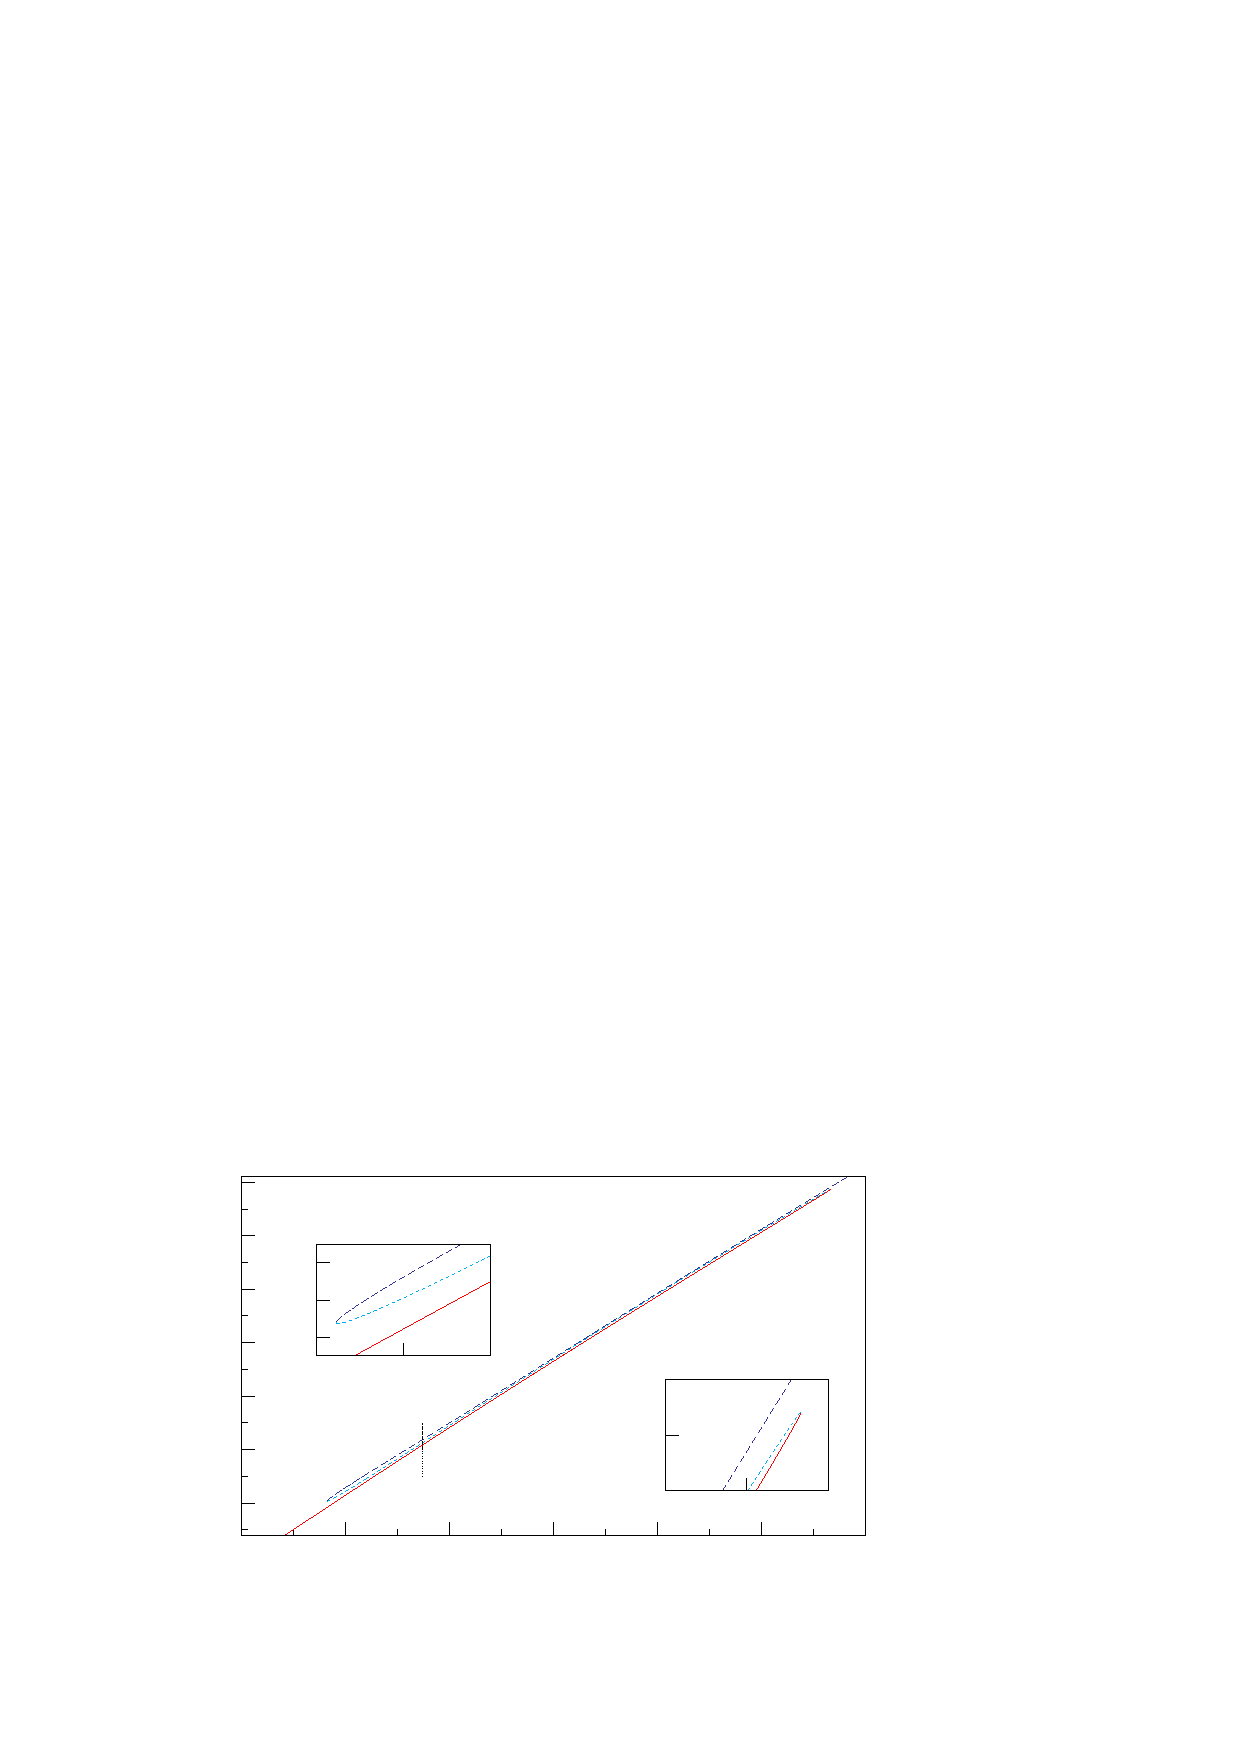
\includegraphics{Images/epslatex/lp_branches}%
\end{picture}%
\begingroup
\setlength{\unitlength}{0.0200bp}%
\begin{picture}(18000,10800)(0,0)%
\put(1925,2420){\makebox(0,0)[r]{\strut{} 23}}%
\put(1925,3704){\makebox(0,0)[r]{\strut{} 24}}%
\put(1925,4987){\makebox(0,0)[r]{\strut{} 25}}%
\put(1925,6271){\makebox(0,0)[r]{\strut{} 26}}%
\put(1925,7554){\makebox(0,0)[r]{\strut{} 27}}%
\put(1925,8838){\makebox(0,0)[r]{\strut{} 28}}%
\put(1925,10122){\makebox(0,0)[r]{\strut{} 29}}%
\put(2200,1100){\makebox(0,0){\strut{} 1.75}}%
\put(4696,1100){\makebox(0,0){\strut{} 1.8}}%
\put(7192,1100){\makebox(0,0){\strut{} 1.85}}%
\put(9688,1100){\makebox(0,0){\strut{} 1.9}}%
\put(12183,1100){\makebox(0,0){\strut{} 1.95}}%
\put(14679,1100){\makebox(0,0){\strut{} 2}}%
\put(17175,1100){\makebox(0,0){\strut{} 2.05}}%
\put(550,5950){\rotatebox{90}{\makebox(0,0){\strut{}$\mathcal{\tilde{D}}$}}}%
\put(9687,275){\makebox(0,0){\strut{}$m$}}%
\put(3725,8185){\makebox(0,0)[r]{\strut{} 23.2}}%
\put(3725,7295){\makebox(0,0)[r]{\strut{} 23.1}}%
\put(3725,6405){\makebox(0,0)[r]{\strut{} 23}}%
\put(8175,5410){\makebox(0,0){\strut{} 1.8}}%
\put(6087,5410){\makebox(0,0){\strut{} 1.795}}%
\put(4000,5410){\makebox(0,0){\strut{} 1.79}}%
\put(12100,5390){\makebox(0,0)[r]{\strut{} 28.9}}%
\put(12100,4055){\makebox(0,0)[r]{\strut{} 28.85}}%
\put(12100,2720){\makebox(0,0)[r]{\strut{} 28.8}}%
\put(16275,2170){\makebox(0,0){\strut{} 2.035}}%
\put(14325,2170){\makebox(0,0){\strut{} 2.03}}%
\put(12375,2170){\makebox(0,0){\strut{} 2.025}}%
\end{picture}%
\endgroup
\endinput

\end{center}
\caption[Branches of bimodals]{\baselineskip=1.0\normalbaselineskip%
Three connected bimodal branches $b_{1}$ (dark blue), $b_{2}$ (light blue) and $b_{3}$ (red) at $\lambda=0.20$ with $\nu={1}\slash{3}$ and $\epsilon=0.1$. From continuation in $m$ the branches $b_{1}$ and $b_{2}$ coalesce at $m=1.791139$, while the $b_{2}$ and $b_{3}$ curves coalesce at $m=2.033325$. The dashed line marks the point at which $b_{2}$ switches from connecting $b_{2}$ and $b_{3}$.}
\label{fig:lp_branches}
\end{figure}
% 
\par % Specifics of one branch
The figure~\ref{fig:lp_branches} shows the continuation of a solution at $m=1.81$, $\lambda=0.20$ in $m$. There are three branches, labelled $b_{1}$, $b_{2}$ and $b_{3}$ connected by two limit points at $lp_{1}=\left(0.2,1.791139\right)$ and $lp_{1}=\left(0.2,2.033325\right)$.  Branch $b_{1}$ can be continued further with $m$ increasing and branch $b_{3}$ be continued in $m$ decreasing. However it is the behaviour of the middle branch $b_{2}$ which is of interest as it connects both branches. 
%
\par
In the neighbourhood of the limit point $lp_{1}$ continuation in $\lambda$ from branch $b_{1}$ reaches a limit point and then heads back on to branch $b_{2}$. Figure~\ref{fig:shell} illustrates the phenomena described: continuation in $\lambda$ (purple) for a range of values of $m$ shows the connection between branches $b_{1}$ (in dark blue) and $b_{2}$ (in light blue). Similarly in the neighbourhood of $lp_{2}$ so the two branches $b_{2}$ and $b_{3}$ (in red) are connected when continuation is performed in $\lambda$. 
%
\begin{figure}[h!tbp]
\begin{center}
%GNUPLOT: LaTeX picture with Postscript
\begin{picture}(0,0)%
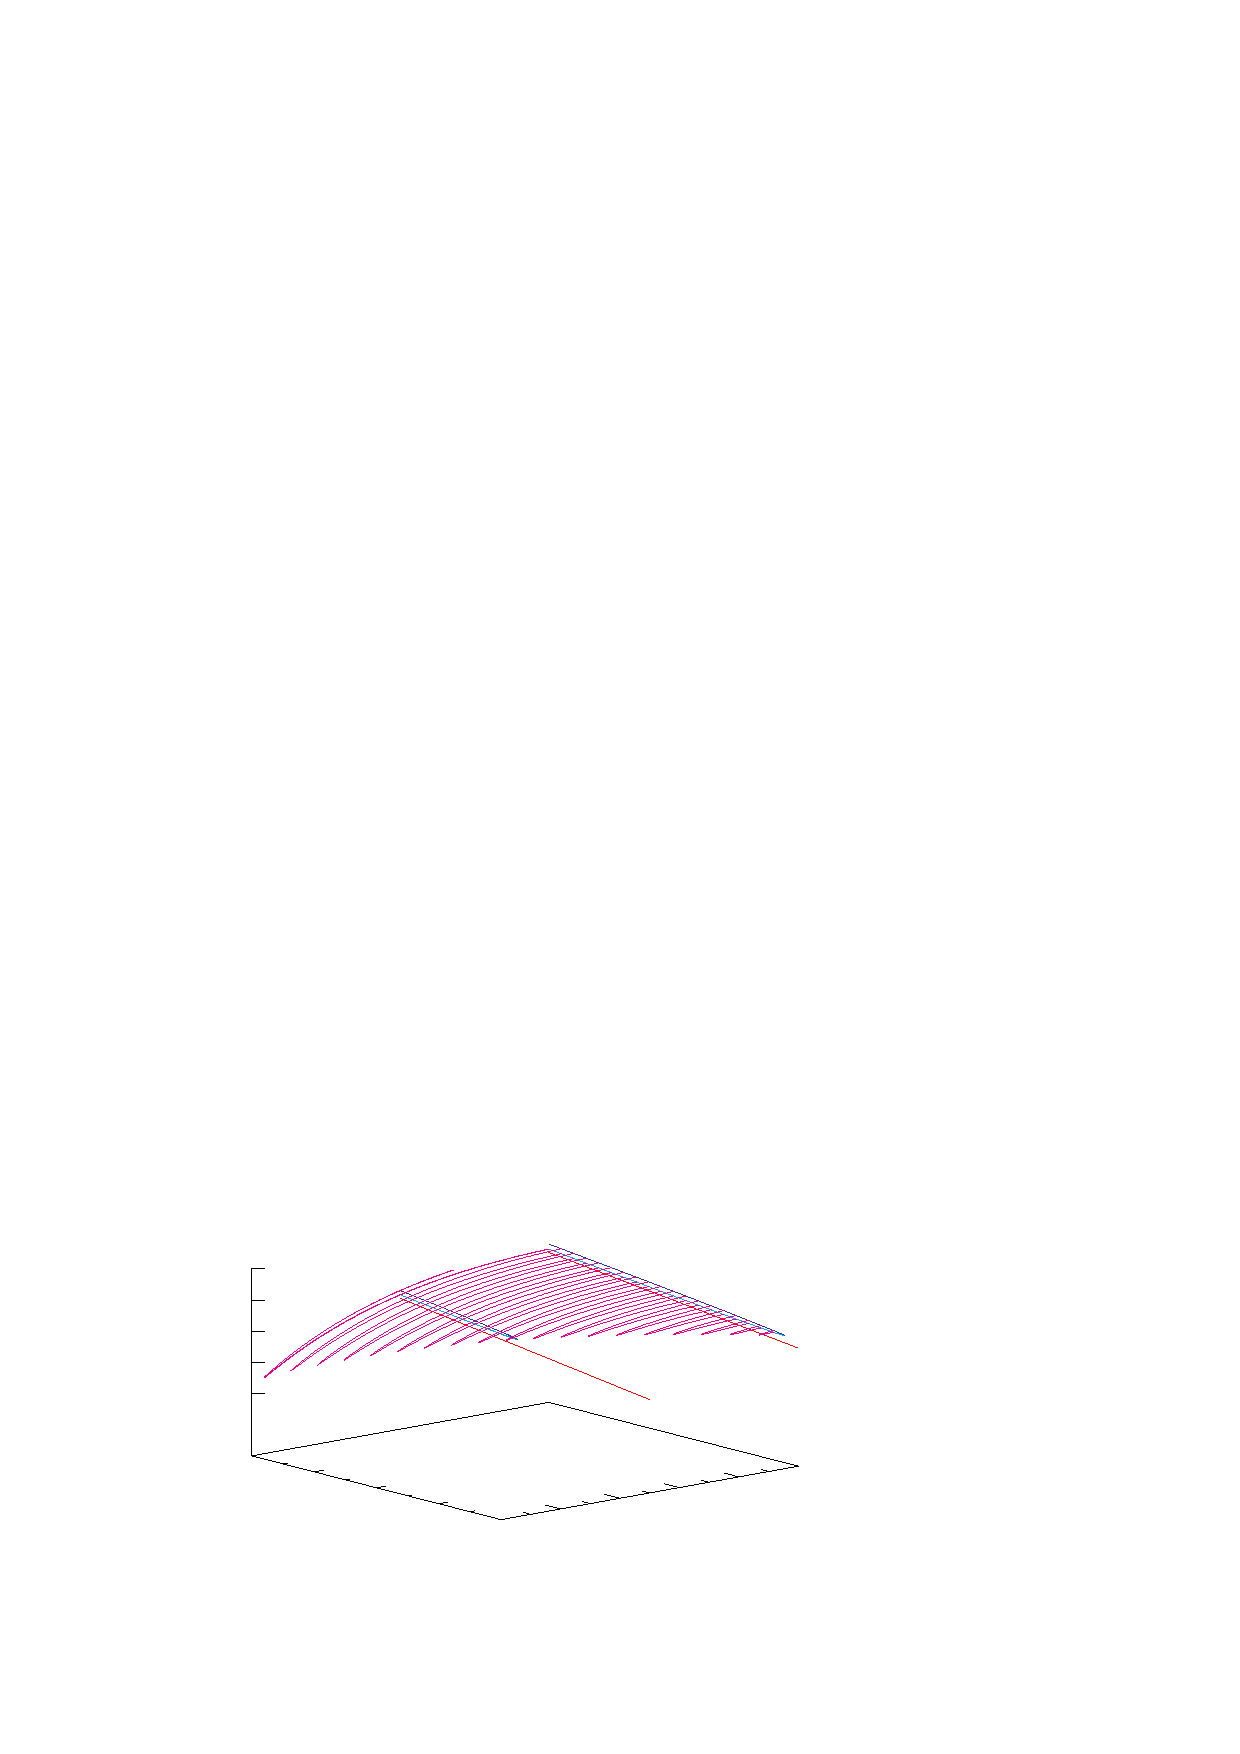
\includegraphics{Images/epslatex/shell}%
\end{picture}%
\begingroup
\setlength{\unitlength}{0.0200bp}%
\begin{picture}(18000,10800)(0,0)%
\put(8762,1852){\makebox(0,0)[l]{\strut{} 0.15}}%
\put(10188,2109){\makebox(0,0)[l]{\strut{} 0.16}}%
\put(11615,2366){\makebox(0,0)[l]{\strut{} 0.17}}%
\put(13042,2623){\makebox(0,0)[l]{\strut{} 0.18}}%
\put(14469,2880){\makebox(0,0)[l]{\strut{} 0.19}}%
\put(15896,3137){\makebox(0,0)[l]{\strut{} 0.2}}%
\put(8216,1948){\makebox(0,0){\strut{} 1.79}}%
\put(6719,2331){\makebox(0,0){\strut{} 1.795}}%
\put(5222,2713){\makebox(0,0){\strut{} 1.8}}%
\put(3726,3096){\makebox(0,0){\strut{} 1.805}}%
\put(2229,3479){\makebox(0,0){\strut{} 1.81}}%
\put(1840,8042){\makebox(0,0)[r]{\strut{} 24}}%
\put(1840,7294){\makebox(0,0)[r]{\strut{} 23.5}}%
\put(1840,6546){\makebox(0,0)[r]{\strut{} 23}}%
\put(1840,5798){\makebox(0,0)[r]{\strut{} 22.5}}%
\put(1840,5051){\makebox(0,0)[r]{\strut{} 22}}%
\put(2439,9164){\makebox(0,0){\strut{}$\tilde{\mathcal{D}}$}}%
\put(13215,1733){\makebox(0,0){\strut{}$\lambda$}}%
\put(3649,2468){\makebox(0,0){\strut{}$m$}}%
\put(2439,9164){\makebox(0,0){\strut{}$\tilde{\mathcal{D}}$}}%
\end{picture}%
\endgroup
\endinput

\end{center}
\caption[Connected branches of bimodals]{\baselineskip=1.0\normalbaselineskip%
Continuation in $m$ and $\lambda$ showing a succession of coalescence curves (purple) connecting the branches $b_{1}$ (dark blue) and $b_{2}$ (light blue) when $\epsilon=0.1$ and $\nu=1\slash{3}$.}
\label{fig:shell}
\end{figure}
%
\par % Limit point switching
Numerical investigation presented in figure~\ref{fig:lambda_many} reveals that when continuation is performed with $\lambda$ decreasing from $\lambda=0.20$, that for $lp_{1}<m<1.837$ the branch $b_{2}$ connects $b_{1}$ (in dark blue) but for $1.837<m<lp_{2}$ the branch $b_{2}$ now connects $b_{3}$ (in red).  The branch $b_{2}$ switches from connecting $b_{1}$ to connecting $b_{3}$. At $m=1.837$ the load-deflection diagrams are minimal, as illustrated by subfigure~\ref{fig:lambda_many_D}.  As shown in subfigure~\ref{fig:lambda_many_T} the truncated arclength is greatest at this point. 
%
\begin{figure}[h!tbp]
\begin{center}
\subfigure[][]{ %GNUPLOT: LaTeX picture with Postscript
\begin{picture}(0,0)%
\includegraphics{Images/epslatex/lambda_many_D}%
\end{picture}%
\begingroup
\setlength{\unitlength}{0.0200bp}%
\begin{picture}(9900,6480)(0,0)%
\put(1925,1650){\makebox(0,0)[r]{\strut{} 12}}%
\put(1925,2126){\makebox(0,0)[r]{\strut{} 14}}%
\put(1925,2601){\makebox(0,0)[r]{\strut{} 16}}%
\put(1925,3077){\makebox(0,0)[r]{\strut{} 18}}%
\put(1925,3552){\makebox(0,0)[r]{\strut{} 20}}%
\put(1925,4028){\makebox(0,0)[r]{\strut{} 22}}%
\put(1925,4503){\makebox(0,0)[r]{\strut{} 24}}%
\put(1925,4979){\makebox(0,0)[r]{\strut{} 26}}%
\put(1925,5454){\makebox(0,0)[r]{\strut{} 28}}%
\put(1925,5930){\makebox(0,0)[r]{\strut{} 30}}%
\put(2200,1100){\makebox(0,0){\strut{} 0.1}}%
\put(3575,1100){\makebox(0,0){\strut{} 0.12}}%
\put(4950,1100){\makebox(0,0){\strut{} 0.14}}%
\put(6325,1100){\makebox(0,0){\strut{} 0.16}}%
\put(7700,1100){\makebox(0,0){\strut{} 0.18}}%
\put(9075,1100){\makebox(0,0){\strut{} 0.2}}%
\put(550,3790){\rotatebox{90}{\makebox(0,0){\strut{}$\tilde{\mathcal{D}}$}}}%
\put(5637,275){\makebox(0,0){\strut{}$\lambda$}}%
\end{picture}%
\endgroup
\endinput
 \label{fig:lambda_many_D} }
\subfigure[][]{ %GNUPLOT: LaTeX picture with Postscript
\begin{picture}(0,0)%
\includegraphics{Images/epslatex/lambda_many_T}%
\end{picture}%
\begingroup
\setlength{\unitlength}{0.0200bp}%
\begin{picture}(9900,6480)(0,0)%
\put(2475,1650){\makebox(0,0)[r]{\strut{} 57}}%
\put(2475,2261){\makebox(0,0)[r]{\strut{} 57.5}}%
\put(2475,2873){\makebox(0,0)[r]{\strut{} 58}}%
\put(2475,3484){\makebox(0,0)[r]{\strut{} 58.5}}%
\put(2475,4096){\makebox(0,0)[r]{\strut{} 59}}%
\put(2475,4707){\makebox(0,0)[r]{\strut{} 59.5}}%
\put(2475,5319){\makebox(0,0)[r]{\strut{} 60}}%
\put(2475,5930){\makebox(0,0)[r]{\strut{} 60.5}}%
\put(2750,1100){\makebox(0,0){\strut{} 0.1}}%
\put(4015,1100){\makebox(0,0){\strut{} 0.12}}%
\put(5280,1100){\makebox(0,0){\strut{} 0.14}}%
\put(6545,1100){\makebox(0,0){\strut{} 0.16}}%
\put(7810,1100){\makebox(0,0){\strut{} 0.18}}%
\put(9075,1100){\makebox(0,0){\strut{} 0.2}}%
\put(550,3790){\rotatebox{90}{\makebox(0,0){\strut{}$\mathcal{T}$}}}%
\put(5912,275){\makebox(0,0){\strut{}$\lambda$}}%
\end{picture}%
\endgroup
\endinput
 \label{fig:lambda_many_T} }
\end{center}
\caption[End shortening and truncation length for bimodals]{\baselineskip=1.0\normalbaselineskip%
Subfigure~\ref{fig:lambda_many_D} shows load deflection diagrams for bimodal configurations for a range of $m$ when continued under $\lambda$. The red curves are those with $m~\ge~1.837$ and thus connect $b_{2}$ to $b_{3}$ whereas the dark blue curves connect $b_{1}$ and $b_{2}$ as $m~\le~1.837$. Subfigure~\ref{fig:lambda_many_T} shows how the truncated arclength increases as the delocalisation increases as $m$ approaches $1.837$ from the left and the right.}  
\label{fig:lambda_many}
\end{figure}
% 
\par % Differing configurations
By the previous coalescence rules, as $b_{1}$ in connected to $b_{2}$ which in turn then connects $b_{3}$, so the two branches $b_{1}$ and $b_{3}$ should be the same. Figure~\ref{fig:xfort} shows the configurations, using the same colour scheme, on the three branches at fixed values of $m$. A number of observations can be made, firstly note that the configurations displayed in subfigures~\ref{fig:xfort.22} and~\ref{fig:xfort.21} and those in subfigures~\ref{fig:xfort.23} and~\ref{fig:xfort.24} are qualitatively similar as the values of $m$ are near the limit points at which they coalesce. Also, it is evident that configurations on branch $b_{1}$ have more quarter turns those on $b_{3}$. It is also clear that on branch $b_{2}$ subfigure~\ref{fig:xfort.21} has the same number of turns as subfigures~\ref{fig:xfort.22} and~\ref{fig:xfort.25} on branch $b_{1}$. Similarly, subfigure~\ref{fig:xfort.23} on branch $b_{2}$ has the same number of turns as subfigures~\ref{fig:xfort.26} and~\ref{fig:xfort.24} on branch $b_{1}$. Thus, the discontinuity the truncation length of the configurations along branch $b_{2}$, as illustrated in subfigure~\ref{fig:lambda_many_T}, is due to an increase the number of quarter turns on the branch of bimodals.
%
\begin{figure}[h!tbp]
\begin{center}
\subfigure[][$b_{1}$, $m=1.80$]{ \input{Images/epslatex/xfort.22.tex} \label{fig:xfort.22} }
\subfigure[][$b_{1}$, $m=2.00$]{ \input{Images/epslatex/xfort.25.tex} \label{fig:xfort.25} }
\subfigure[][$b_{2}$, $m=1.80$]{ \input{Images/epslatex/xfort.21.tex} \label{fig:xfort.21} }
\subfigure[][$b_{2}$, $m=2.00$]{ \input{Images/epslatex/xfort.23.tex} \label{fig:xfort.23} }
\subfigure[][$b_{3}$, $m=1.80$]{ \input{Images/epslatex/xfort.26.tex} \label{fig:xfort.26} }
\subfigure[][$b_{3}$, $m=2.00$]{ \input{Images/epslatex/xfort.24.tex} \label{fig:xfort.24} }
\end{center}
\caption[Bimodal configurations on connected branches]{\baselineskip=1.0\normalbaselineskip%
Bimodal configurations on the connected branches in figure~\ref{fig:lp_branches}.}  
\label{fig:xfort}
\end{figure}
% 
\par % Other branches
Branch $b_{3}$ then approaches $\lambda_{c}^{\left(2\right)}$ and passes beyond it merging with other isolae. The branches $b_{2}$ and $b_{1}$ cannot pass through the codimension-two point  and instead reach limit points.  In order to merge with other branches branches $b_{1}$ and $b_{2}$ must be continued in $m$ onto branch $b_{3}$, as in figure~\ref{fig:lp}. As has been observed, the branch $b_{3}$ appears to have a fewer number quarter turns than branches $b_{2}$ and $b_{1}$ and, as was seen in figure~\ref{fig:bi_lp} in the anisotropic Kirchhoff rod, bimodals with smaller gaps between localisations can be continued further towards the codimension-two point.
%
\par 
While the results presented here hold for other bimodals, without analytical results the numerical evidence provides an insight into one branch in a multiplicity of homoclinic solutions.  A rich bifurcation structure clearly exists, for example, just beyond $lp_{2}$ the branch $b_{1}$ connects, through continuation in $\lambda$, with another distinct branch at $\left(0.2,1.975411\right)$. This new branch possesses limit points both forward and backward in $m$ and its load-deflection diagrams do not resemble figure~\ref{fig:lp_branches}.
%
\par % Spectrum of limit points
The $\left(\lambda,m\right)$ parameter space was explored and collection of limit points discovered. The results are presented in figure~\ref{fig:spectrum}. Again, note the figure may not give an global picture of the bifurcation structure of the bimodals as continuation was performed manually from a single solution. It should be noted that in this figure the only limit points which are expected (from linear analysis) are those which approach the buckling line such as $lp_{1}$ rather than those which are away from the buckling line such as $lp_{2}$. A similar set of results should be expected for solutions with small $\lambda$ to the left of the elliptic region, but pairs of limit points should be expected one approaching the buckling line another in the anti-integrable limit.
% 
\begin{figure}[h!tbp]
\begin{center}
\subfigure[][$m=1.81$]{
%GNUPLOT: LaTeX picture with Postscript
\begin{picture}(0,0)%
\includegraphics{Images/epslatex/R_cusp}%
\end{picture}%
\begingroup
\setlength{\unitlength}{0.0200bp}%
\begin{picture}(9900,6480)(0,0)%
\put(2200,1650){\makebox(0,0)[r]{\strut{} 1}}%
\put(2200,2261){\makebox(0,0)[r]{\strut{} 1.1}}%
\put(2200,2873){\makebox(0,0)[r]{\strut{} 1.2}}%
\put(2200,3484){\makebox(0,0)[r]{\strut{} 1.3}}%
\put(2200,4096){\makebox(0,0)[r]{\strut{} 1.4}}%
\put(2200,4707){\makebox(0,0)[r]{\strut{} 1.5}}%
\put(2200,5319){\makebox(0,0)[r]{\strut{} 1.6}}%
\put(2200,5930){\makebox(0,0)[r]{\strut{} 1.7}}%
\put(3192,1100){\makebox(0,0){\strut{} 0.15}}%
\put(4627,1100){\makebox(0,0){\strut{} 0.2}}%
\put(6062,1100){\makebox(0,0){\strut{} 0.25}}%
\put(7497,1100){\makebox(0,0){\strut{} 0.3}}%
\put(8932,1100){\makebox(0,0){\strut{} 0.35}}%
\put(550,3790){\rotatebox{90}{\makebox(0,0){\strut{}$\tilde{\mathcal{R}}$}}}%
\put(5775,275){\makebox(0,0){\strut{}$\lambda$}}%
\end{picture}%
\endgroup
\endinput

%GNUPLOT: LaTeX picture with Postscript
\begin{picture}(0,0)%
\includegraphics{Images/epslatex/D_cusp}%
\end{picture}%
\begingroup
\setlength{\unitlength}{0.0200bp}%
\begin{picture}(9900,6480)(0,0)%
\put(2475,1650){\makebox(0,0)[r]{\strut{} 21.6}}%
\put(2475,2078){\makebox(0,0)[r]{\strut{} 21.8}}%
\put(2475,2506){\makebox(0,0)[r]{\strut{} 22}}%
\put(2475,2934){\makebox(0,0)[r]{\strut{} 22.2}}%
\put(2475,3362){\makebox(0,0)[r]{\strut{} 22.4}}%
\put(2475,3790){\makebox(0,0)[r]{\strut{} 22.6}}%
\put(2475,4218){\makebox(0,0)[r]{\strut{} 22.8}}%
\put(2475,4646){\makebox(0,0)[r]{\strut{} 23}}%
\put(2475,5074){\makebox(0,0)[r]{\strut{} 23.2}}%
\put(2475,5502){\makebox(0,0)[r]{\strut{} 23.4}}%
\put(2475,5930){\makebox(0,0)[r]{\strut{} 23.6}}%
\put(3438,1100){\makebox(0,0){\strut{} 0.15}}%
\put(4813,1100){\makebox(0,0){\strut{} 0.2}}%
\put(6188,1100){\makebox(0,0){\strut{} 0.25}}%
\put(7563,1100){\makebox(0,0){\strut{} 0.3}}%
\put(8938,1100){\makebox(0,0){\strut{} 0.35}}%
\put(550,3790){\rotatebox{90}{\makebox(0,0){\strut{}$\tilde{\mathcal{D}}$}}}%
\put(5912,275){\makebox(0,0){\strut{}$\lambda$}}%
\end{picture}%
\endgroup
\endinput
 \label{fig:cusp} }
\subfigure[][$m=1.91$]{
%GNUPLOT: LaTeX picture with Postscript
\begin{picture}(0,0)%
\includegraphics{Images/epslatex/R_coalescence}%
\end{picture}%
\begingroup
\setlength{\unitlength}{0.0200bp}%
\begin{picture}(9900,6480)(0,0)%
\put(2475,1650){\makebox(0,0)[r]{\strut{} 0.55}}%
\put(2475,2185){\makebox(0,0)[r]{\strut{} 0.6}}%
\put(2475,2720){\makebox(0,0)[r]{\strut{} 0.65}}%
\put(2475,3255){\makebox(0,0)[r]{\strut{} 0.7}}%
\put(2475,3790){\makebox(0,0)[r]{\strut{} 0.75}}%
\put(2475,4325){\makebox(0,0)[r]{\strut{} 0.8}}%
\put(2475,4860){\makebox(0,0)[r]{\strut{} 0.85}}%
\put(2475,5395){\makebox(0,0)[r]{\strut{} 0.9}}%
\put(2475,5930){\makebox(0,0)[r]{\strut{} 0.95}}%
\put(2750,1100){\makebox(0,0){\strut{} 0.095}}%
\put(3804,1100){\makebox(0,0){\strut{} 0.1}}%
\put(4858,1100){\makebox(0,0){\strut{} 0.105}}%
\put(5913,1100){\makebox(0,0){\strut{} 0.11}}%
\put(6967,1100){\makebox(0,0){\strut{} 0.115}}%
\put(8021,1100){\makebox(0,0){\strut{} 0.12}}%
\put(9075,1100){\makebox(0,0){\strut{} 0.125}}%
\put(550,3790){\rotatebox{90}{\makebox(0,0){\strut{}$\tilde{\mathcal{R}}$}}}%
\put(5912,275){\makebox(0,0){\strut{}$\lambda$}}%
\end{picture}%
\endgroup
\endinput
 
%GNUPLOT: LaTeX picture with Postscript
\begin{picture}(0,0)%
\includegraphics{Images/epslatex/D_coalescence}%
\end{picture}%
\begingroup
\setlength{\unitlength}{0.0200bp}%
\begin{picture}(9900,6480)(0,0)%
\put(1925,1650){\makebox(0,0)[r]{\strut{} 15}}%
\put(1925,2126){\makebox(0,0)[r]{\strut{} 16}}%
\put(1925,2601){\makebox(0,0)[r]{\strut{} 17}}%
\put(1925,3077){\makebox(0,0)[r]{\strut{} 18}}%
\put(1925,3552){\makebox(0,0)[r]{\strut{} 19}}%
\put(1925,4028){\makebox(0,0)[r]{\strut{} 20}}%
\put(1925,4503){\makebox(0,0)[r]{\strut{} 21}}%
\put(1925,4979){\makebox(0,0)[r]{\strut{} 22}}%
\put(1925,5454){\makebox(0,0)[r]{\strut{} 23}}%
\put(1925,5930){\makebox(0,0)[r]{\strut{} 24}}%
\put(2200,1100){\makebox(0,0){\strut{} 0.095}}%
\put(3346,1100){\makebox(0,0){\strut{} 0.1}}%
\put(4492,1100){\makebox(0,0){\strut{} 0.105}}%
\put(5638,1100){\makebox(0,0){\strut{} 0.11}}%
\put(6783,1100){\makebox(0,0){\strut{} 0.115}}%
\put(7929,1100){\makebox(0,0){\strut{} 0.12}}%
\put(9075,1100){\makebox(0,0){\strut{} 0.125}}%
\put(550,3790){\rotatebox{90}{\makebox(0,0){\strut{}$\tilde{\mathcal{D}}$}}}%
\put(5637,275){\makebox(0,0){\strut{}$\lambda$}}%
\end{picture}%
\endgroup
\endinput
 \label{fig:coalescence} }
\subfigure[][$m=2.00$]{
%GNUPLOT: LaTeX picture with Postscript
\begin{picture}(0,0)%
\includegraphics{Images/epslatex/R_dovetail}%
\end{picture}%
\begingroup
\setlength{\unitlength}{0.0200bp}%
\begin{picture}(9900,6480)(0,0)%
\put(2200,1650){\makebox(0,0)[r]{\strut{} 0.8}}%
\put(2200,2126){\makebox(0,0)[r]{\strut{} 0.9}}%
\put(2200,2601){\makebox(0,0)[r]{\strut{} 1}}%
\put(2200,3077){\makebox(0,0)[r]{\strut{} 1.1}}%
\put(2200,3552){\makebox(0,0)[r]{\strut{} 1.2}}%
\put(2200,4028){\makebox(0,0)[r]{\strut{} 1.3}}%
\put(2200,4503){\makebox(0,0)[r]{\strut{} 1.4}}%
\put(2200,4979){\makebox(0,0)[r]{\strut{} 1.5}}%
\put(2200,5454){\makebox(0,0)[r]{\strut{} 1.6}}%
\put(2200,5930){\makebox(0,0)[r]{\strut{} 1.7}}%
\put(2475,1100){\makebox(0,0){\strut{} 0.1}}%
\put(3795,1100){\makebox(0,0){\strut{} 0.15}}%
\put(5115,1100){\makebox(0,0){\strut{} 0.2}}%
\put(6435,1100){\makebox(0,0){\strut{} 0.25}}%
\put(7755,1100){\makebox(0,0){\strut{} 0.3}}%
\put(9075,1100){\makebox(0,0){\strut{} 0.35}}%
\put(550,3790){\rotatebox{90}{\makebox(0,0){\strut{}$\tilde{\mathcal{R}}$}}}%
\put(5775,275){\makebox(0,0){\strut{}$\lambda$}}%
\end{picture}%
\endgroup
\endinput

%GNUPLOT: LaTeX picture with Postscript
\begin{picture}(0,0)%
\includegraphics{Images/epslatex/D_dovetail}%
\end{picture}%
\begingroup
\setlength{\unitlength}{0.0200bp}%
\begin{picture}(9900,6480)(0,0)%
\put(2475,1650){\makebox(0,0)[r]{\strut{} 24.5}}%
\put(2475,2126){\makebox(0,0)[r]{\strut{} 25}}%
\put(2475,2601){\makebox(0,0)[r]{\strut{} 25.5}}%
\put(2475,3077){\makebox(0,0)[r]{\strut{} 26}}%
\put(2475,3552){\makebox(0,0)[r]{\strut{} 26.5}}%
\put(2475,4028){\makebox(0,0)[r]{\strut{} 27}}%
\put(2475,4503){\makebox(0,0)[r]{\strut{} 27.5}}%
\put(2475,4979){\makebox(0,0)[r]{\strut{} 28}}%
\put(2475,5454){\makebox(0,0)[r]{\strut{} 28.5}}%
\put(2475,5930){\makebox(0,0)[r]{\strut{} 29}}%
\put(2750,1100){\makebox(0,0){\strut{} 0.1}}%
\put(4015,1100){\makebox(0,0){\strut{} 0.15}}%
\put(5280,1100){\makebox(0,0){\strut{} 0.2}}%
\put(6545,1100){\makebox(0,0){\strut{} 0.25}}%
\put(7810,1100){\makebox(0,0){\strut{} 0.3}}%
\put(9075,1100){\makebox(0,0){\strut{} 0.35}}%
\put(550,3790){\rotatebox{90}{\makebox(0,0){\strut{}$\tilde{\mathcal{D}}$}}}%
\put(5912,275){\makebox(0,0){\strut{}$\lambda$}}%
\end{picture}%
\endgroup
\endinput
 \label{fig:dovetail} }
\caption[Load-deflections]{\baselineskip=1.0\normalbaselineskip%
A variety of load-deflection diagrams for $\lambda$ showing different classes of bifurcation diagram.}
\label{fig:load_deflections}
\end{center}
\end{figure}
% 
\begin{figure}[h!tbp]
\begin{center}
%GNUPLOT: LaTeX picture with Postscript
\begin{picture}(0,0)%
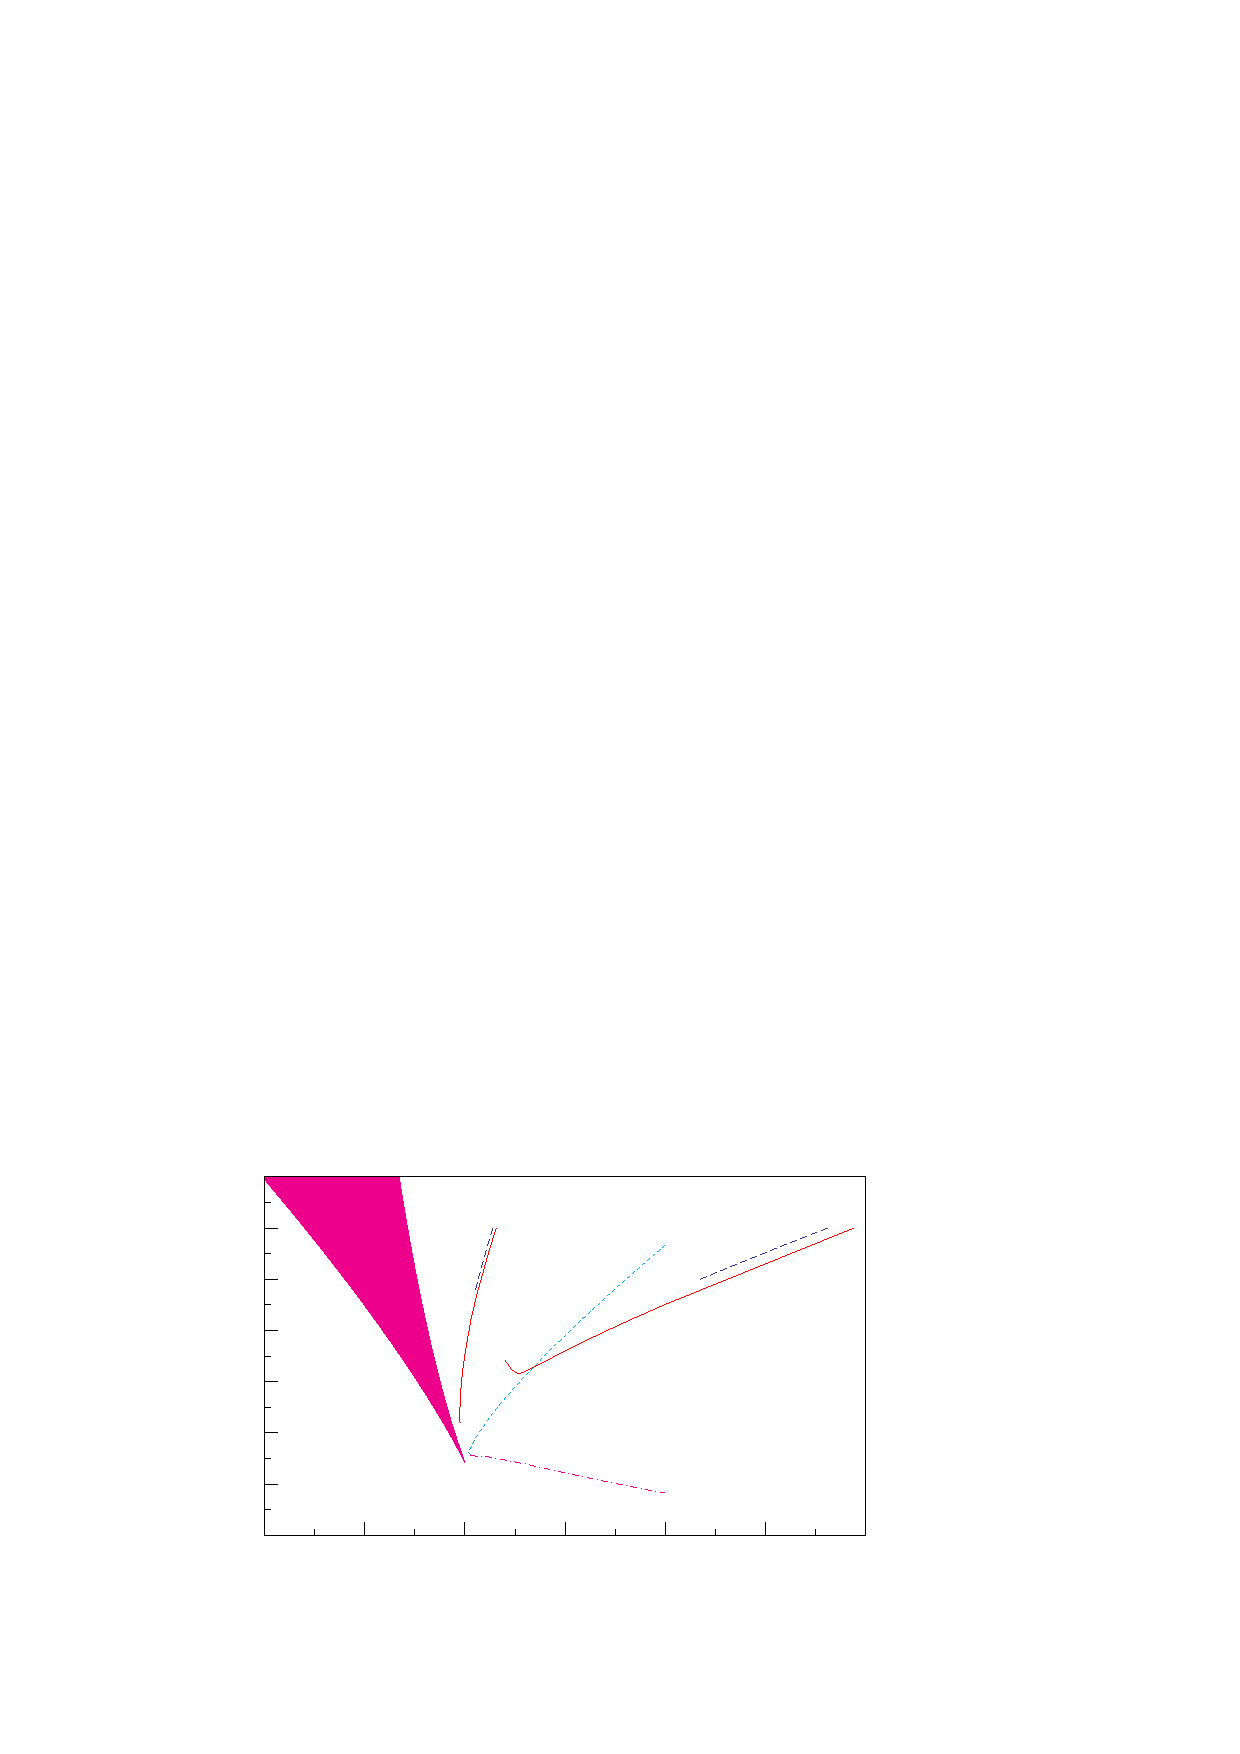
\includegraphics{Images/epslatex/spectrum}%
\end{picture}%
\begingroup
\setlength{\unitlength}{0.0200bp}%
\begin{picture}(18000,10800)(0,0)%
\put(2475,1650){\makebox(0,0)[r]{\strut{} 1.75}}%
\put(2475,2879){\makebox(0,0)[r]{\strut{} 1.8}}%
\put(2475,4107){\makebox(0,0)[r]{\strut{} 1.85}}%
\put(2475,5336){\makebox(0,0)[r]{\strut{} 1.9}}%
\put(2475,6564){\makebox(0,0)[r]{\strut{} 1.95}}%
\put(2475,7793){\makebox(0,0)[r]{\strut{} 2}}%
\put(2475,9021){\makebox(0,0)[r]{\strut{} 2.05}}%
\put(2475,10250){\makebox(0,0)[r]{\strut{} 2.1}}%
\put(2750,1100){\makebox(0,0){\strut{} 0}}%
\put(5154,1100){\makebox(0,0){\strut{} 0.05}}%
\put(7558,1100){\makebox(0,0){\strut{} 0.1}}%
\put(9963,1100){\makebox(0,0){\strut{} 0.15}}%
\put(12367,1100){\makebox(0,0){\strut{} 0.2}}%
\put(14771,1100){\makebox(0,0){\strut{} 0.25}}%
\put(17175,1100){\makebox(0,0){\strut{} 0.3}}%
\put(550,5950){\rotatebox{90}{\makebox(0,0){\strut{}$m$}}}%
\put(9962,275){\makebox(0,0){\strut{}$\lambda$}}%
\end{picture}%
\endgroup
\endinput
 % ...auto/Magnetic/LP/Data
\end{center}
\caption[Limit points of a bimodal]{\baselineskip=1.0\normalbaselineskip%
A succession of limit points for a set of bimodals against the spectrum of Floquet multipliers when $\epsilon=0.1$ and $\nu=1\slash{3}$. As in figure~\ref{fig:lambda_spectrum} the shaded area is the elliptic regime and the dotted line the codimension-one curve~\eqref{eq:codim_one_curve}.}
\label{fig:spectrum}
\end{figure}